% Pre-ambulo
\documentclass[a4paper, 12pt]{abnt}

\usepackage[brazil]{babel}
\usepackage[utf8]{inputenc}
\usepackage[T1]{fontenc}
\usepackage{lmodern}


\usepackage[
    bookmarksdepth=4,
    bookmarksopen=true,
    bookmarksnumbered=true,
    colorlinks=true,
    allcolors=black,
    linktoc=all,
    pdfborder={0 0 0},
    breaklinks=true
]{hyperref}
\usepackage{bookmark}

\hypersetup{
    pdftitle={Hiperpersonalização em Gêmeos Digitais Urbanos: uma Camada de Orquestração Sensível ao Contexto para Notificação e Resposta a Emergências},
    pdfauthor={Alexandre Cesar de Oliveira Guimarães},
    pdfsubject={Qualificação de Mestrado -- PPgTI/IMD/UFRN},
    pdfkeywords={Gêmeos Digitais Urbanos; NGSI-LD; FIWARE; Data Spaces; Hiperpersonalização; Sensibilidade ao Contexto}
}

\usepackage{dsfont}
\usepackage{amssymb,amsmath}
\usepackage{multirow}
\usepackage[alf]{abntcite}

\makeatletter
\renewcommand{\citeoption}[1]{}
\makeatother
\usepackage[pdftex]{color, graphicx}
\usepackage{colortbl}
\usepackage{url}
\usepackage{abnt-alf}
\usepackage{abntcite}
\usepackage{algorithm}
\usepackage{algorithmic}
%\usepackage{alg}


% Redefinicao de instrucoes
\floatname{algorithm}{Algoritmo}
\renewcommand{\algorithmicrequire}{\textbf{Entrada:}}
\renewcommand{\algorithmicensure}{\textbf{Saída:}}
\renewcommand{\algorithmicend}{\textbf{fim}}
\renewcommand{\algorithmicif}{\textbf{se}}
\renewcommand{\algorithmicthen}{\textbf{então}}
\renewcommand{\algorithmicelse}{\textbf{senão}}
\renewcommand{\algorithmicfor}{\textbf{para}}
\renewcommand{\algorithmicforall}{\textbf{para todo}}
\renewcommand{\algorithmicdo}{\textbf{faça}}
\renewcommand{\algorithmicwhile}{\textbf{enquanto}}
\renewcommand{\algorithmicloop}{\textbf{loop}}
\renewcommand{\algorithmicrepeat}{\textbf{repetir}}
\renewcommand{\algorithmicuntil}{\textbf{até que}}
\renewcommand{\algorithmiccomment}[1]{\% #1}


% Definicao da lista de simbolos
% \simb[entrada na lista de simbolos]{simbolo}:
% Escreve o simbolo no texto e uma entrada na lista de simbolos.
% Se o parametro opcional e omitido, usa-se o parametro obrigatorio.
\newcommand{\simb}[2][]
{%
	\ifthenelse{\equal{#1}{}}
	{\addcontentsline{los}{simbolo}{#2}}
	{\addcontentsline{los}{simbolo}{#1}}#2
}
% Para aceitar comandos com @ (at) no nome
\makeatletter 
% \listadesimbolos: comando que imprime a lista de simbolos
\newcommand{\listadesimbolos}
{
	\pretextualchapter{Lista de símbolos}
	{\setlength{\parindent}{0cm}
	\@starttoc{los}}
}
% Como a entrada sera impressa
\newcommand\l@simbolo[2]{\par #1}
\makeatother


% Definicao da lista de abreviaturas e siglas
% \abrv[entrada na lista de simbolos]{abreviatura}:
% Escreve a sigla/abreviatura no texto e uma entrada na lista de abreviaturas e siglas.
% Se o parametro opcional e omitido, usa-se o parametro obrigatorio.
\newcommand{\abrv}[2][]
{%
	\ifthenelse{\equal{#1}{}}
	{\addcontentsline{loab}{abreviatura}{#2}}
	{\addcontentsline{loab}{abreviatura}{#1}}#2
}
% Para aceitar comandos com @ (at) no nome
\makeatletter 
% \listadeabreviaturas: comando que imprime a lista de abreviaturas e siglas
\newcommand{\listadeabreviaturas}
{
	\pretextualchapter{Lista de abreviaturas e siglas}
	{\setlength{\parindent}{0cm}
	\@starttoc{loab}}
}
% Como a entrada sera impressa
\newcommand\l@abreviatura[2]{\par #1}
\makeatother


% \listofalgorithms: comando que imprime a lista de algoritmos
\renewcommand{\listalgorithmname}{Lista de algoritmos}


% Hifenização de palavras feita de forma incorreta pelo LaTeX
\hyphenation{PYTHON ou-tros}


\usepackage{tabularx}
\usepackage{float} % [H] fixa a tabela junto da citacao
\usepackage{booktabs}
\usepackage{longtable}
\usepackage{listings}
\usepackage{enumitem}

% Cores para os trechos de codigo (definidas via 'color', ja carregado)
\definecolor{codebg}{rgb}{0.97,0.97,0.97}
\definecolor{codegray}{rgb}{0.45,0.45,0.45}
\definecolor{codekey}{rgb}{0.0,0.0,0.55}
\definecolor{codestr}{rgb}{0.0,0.35,0.0}

\lstdefinestyle{jsonld}{
	backgroundcolor=\color{codebg},
	basicstyle=\ttfamily\footnotesize,
	commentstyle=\color{codegray}\itshape,
	keywordstyle=\color{codekey}\bfseries,
	stringstyle=\color{codestr},
	breaklines=true,
	breakatwhitespace=false,
	breakindent=1.4em,
	postbreak=\mbox{\textcolor{codegray}{$\hookrightarrow$}\space},
	frame=single,
	numbers=left,
	numberstyle=\tiny\color{codegray},
	tabsize=2,
	showstringspaces=false,
	captionpos=b
}
\lstset{style=jsonld}
\renewcommand{\lstlistingname}{Listagem}
\renewcommand{\lstlistlistingname}{Lista de listagens}

% Legenda de fonte para figuras/tabelas ("Fonte: ...")
\newcommand{\legend}[1]{{\footnotesize #1\par}}
% Cabecalho girado 90 graus para colunas estreitas (texto por extenso, em ate duas linhas)
\newcommand{\hdrv}[1]{\rotatebox[origin=lB]{90}{\begin{tabular}[b]{@{}l@{}}\bfseries #1\end{tabular}}}

% Marca visivel de pendencia de verificacao; \pendenciasfalse oculta todas as marcas
\newif\ifpendencias\pendenciasfalse
\newcommand{\pend}[1]{\ifpendencias\textbf{[#1]}\fi}



% Inicio do documento
\begin{document}

% Parametros de posicionamento de float: evitam que tabelas grandes sejam
% adiadas varias paginas, o que deixava paginas pela metade no Capitulo 4.
\renewcommand{\topfraction}{0.88}
\renewcommand{\bottomfraction}{0.70}
\renewcommand{\textfraction}{0.10}
\renewcommand{\floatpagefraction}{0.75}
\setcounter{topnumber}{3}
\setcounter{bottomnumber}{2}
\setcounter{totalnumber}{4}


	\frenchspacing

	% Capa (arquivo Includes/Capa.tex)
	% Capa
% Protecao externa do trabalho e sobre a qual se imprimem as informacoes
% indispensaveis a sua identificacao.

\begin{titlepage}
	\begin{center}

		% Cabecalho: brasao da Universidade, logotipo do Instituto e dados
		% de vinculacao do aluno (Universidade, Instituto e Programa).
		%
		% NOTA AO AUTOR: o logotipo abaixo (Logotipo-DIMAp.png) pertence ao
		% Departamento de Informatica e Matematica Aplicada (DIMAp), herdado
		% do modelo-base do PPgSC, e NAO corresponde ao Instituto Metropole
		% Digital (IMD/PPgTI). Substitua pelo logotipo oficial do IMD antes
		% de submeter o documento.
		\begin{minipage}{2.3cm}
			\begin{center}
				
\includegraphics[width=2.25cm, height=2.68cm]{Imagens/Brasao-UFRN.jpg}
			\end{center}
		\end{minipage}
		\begin{minipage}{11.15cm}
			\begin{center}
				\begin{espacosimples}
					{\small \ \\
                       \textsc{Universidade Federal do Rio Grande do Norte}		\\
					   \textsc{Instituto Metrópole Digital}						\\
					   \textsc{Programa de Pós-Graduação em Tecnologia da Informação} \\
                       \textsc{Mestrado Profissional em Tecnologia da Informação}}		\\
				\end{espacosimples}
			\end{center}
		\end{minipage}
		\begin{minipage}{2.3cm}
			\begin{center}
				
\includegraphics[width=2.25cm, height=2.68cm]{Imagens/Brasao-PPgTi.png}
			\end{center}
		\end{minipage}

		\vspace{6cm}

		% Titulo do trabalho
		{\setlength{\baselineskip}%
		{1.3\baselineskip} {\LARGE \textbf{Hiperpersonalização em Gêmeos Digitais Urbanos: uma Camada de Orquestração Sensível ao Contexto para Notificação e Resposta a Emergências}}\par}

		\vspace{3cm}

		% Nome do aluno (autor)
		{\large \textbf{Alexandre Cesar de Oliveira Guimarães}}

		\vspace{6cm}

		% Local da instituicao e data de entrega
		Natal-RN\\Outubro de 2026
	\end{center}
\end{titlepage}


	% Folha de rosto (arquivo Includes/FolhaRosto.tex)
	% Folha de rosto
% Contem os elementos essenciais a identificacao do trabalho.

% Titulo, nome do aluno e respectivo orientador e filiacao
\titulo{\Large{Hiperpersonalização em Gêmeos Digitais Urbanos: uma Camada de Orquestração Sensível ao Contexto para Notificação e Resposta a Emergências}} \autor{Alexandre Cesar de Oliveira Guimarães} \orientador[Orientador]{\par Prof.\ Dr.\ Frederico Araujo da Silva Lopes} \instituicao { PPgTI -- Programa de Pós-Graduação em Tecnologia da Informação\par
	IMD -- Instituto Metrópole Digital\par
	UFRN -- Universidade Federal do Rio Grande do Norte }

% Natureza do trabalho (nao deve ser modificada)
\comentario { Documento de Exame de Qualificação apresentado ao Programa de Pós-Graduação em Tecnologia da Informação do Instituto Metrópole Digital da Universidade Federal do Rio Grande do Norte, como requisito parcial para a obtenção do título de Mestre em Tecnologia da Informação.\bigskip\\
   \textit{Linha de pesquisa}:\\Engenharia de Software e Sistemas de Informação aplicados a Cidades Inteligentes e Gêmeos Digitais Urbanos }

% Local e data
\local{Natal-RN} \data{Outubro de 2026}

\folhaderosto


	% Folha de aprovacao (arquivo Includes/FolhaAprovacao.tex)
	% Folha de aprovacao
%
% NOTA AO AUTOR: os membros da banca examinadora do Exame de Qualificação
% ainda nao foram definidos no documento original. Preencha os nomes e
% filiacoes reais abaixo antes de submeter (mantendo o orientador como
% presidente).
\begin{folhadeaprovacao}
	\setlength{\ABNTsignthickness}{0.4pt}
	\setlength{\ABNTsignwidth}{10cm}

	\noindent
	Documento de Exame de Qualificação sob o título \textit{Hiperpersonalização em Gêmeos Digitais Urbanos: uma Camada de Orquestração Sensível ao Contexto para Notificação e Resposta a Emergências}, apresentado por Alexandre Cesar de Oliveira Guimarães e avaliado pelo Programa de Pós-Graduação em Tecnologia da Informação do Instituto Metrópole Digital da Universidade Federal do Rio Grande do Norte, sendo aprovado por todos os membros da banca examinadora abaixo especificada:

	\assinatura { Prof.\ Dr.\ Frederico Araujo da Silva Lopes \\
		{\small Presidente (Orientador)}											          \smallskip\\
		{\footnotesize IMD -- Instituto Metrópole Digital		   \\
		  	UFRN -- Universidade Federal do Rio Grande do Norte } }

   \assinatura { Nome completo do membro interno da banca \\
		{\small Membro Interno}											          \smallskip\\
		{\footnotesize IMD -- Instituto Metrópole Digital		   \\
		  	UFRN -- Universidade Federal do Rio Grande do Norte } }

   \assinatura { Nome completo do membro externo da banca \\
		{\small Membro Externo}											          \smallskip\\
		{\footnotesize Instituição do membro externo } }

	\begin{center}
		Natal-RN, \rule[-0.3ex]{2.5cm}{0.4pt} de Outubro de 2026.
	\end{center}
\end{folhadeaprovacao}


	% % Dedicatoria (arquivo Includes/Dedicatoria.tex)
	% % Dedicatoria
%
% NOTA AO AUTOR: espaco opcional e pessoal -- substitua o texto abaixo
% pela dedicatoria real, se desejar incluir uma.

\chapter*{}
\vspace{15cm}
\begin{flushright}
	\textit{Espaço reservado para a dedicatória do autor (opcional -- substituir ou remover).}
\end{flushright}


	% % Agradecimentos (arquivo Includes/Agradecimentos.tex)
	% % Agradecimentos
%
% NOTA AO AUTOR: espaco opcional e pessoal -- substitua pelos
% agradecimentos reais (orientador, PPgTI/IMD, colegas de pesquisa,
% agencias de fomento com respectivo numero de processo, se houver).

\chapter*{Agradecimentos}

Espaço reservado para os agradecimentos do autor (opcional -- substituir pelo texto definitivo).


	% % Epigrafe (arquivo Includes/Epigrafe.tex)
	% % Epigrafe (citacao seguida de indicacao de autoria)
%
% NOTA AO AUTOR: espaco opcional e pessoal -- substitua pela epigrafe
% real, se desejar incluir uma.

\chapter*{}
\vspace{15cm}
\begin{flushright}
	\textit { Espaço reservado para a epígrafe (opcional -- substituir ou remover). }\medskip\\
	Autor
\end{flushright}


	% Resumo em lingua vernacula (arquivo Includes/Resumo.tex)
	% Resumo em lingua vernacula
\begin{center}
	{\Large{\textbf{Hiperpersonalização em Gêmeos Digitais Urbanos: uma Camada de Orquestração Sensível ao Contexto para Notificação e Resposta a Emergências}}}
\end{center}

\vspace{1cm}

\begin{flushright}
	Autor: Alexandre Cesar de Oliveira Guimarães\\
	Orientador: Prof.\ Dr.\ Frederico Araujo da Silva Lopes
\end{flushright}

\vspace{1cm}

\begin{center}
	\Large{\textsc{\textbf{Resumo}}}
\end{center}

\noindent Os gêmeos digitais urbanos deixaram de ser maquetes tridimensionais e
tornaram-se plataformas de dados em operação nas cidades. Cada vez mais, essas plataformas trazem com fidelidade a infraestrutura urbana, suas vias, edificações e dados de forma geral, mas tratam as pessoas como agregado estatístico, e não como entidades objeto de definição de contexto. A limitação se revela quando o sistema precisa agir sobre indivíduos, e não sobre a média deles. Numa emergência, a informação poderia ser direcionada a quem tem perfil competente para atuar, enquanto cada pessoa afetada receberia a orientação pertinente à sua própria condição; sem perfil no modelo de contexto, porém, a plataforma só é capaz de emitir a mesma mensagem para todos. O mapeamento sistemático da literatura conduzido neste trabalho mostra que a limitação é do campo, e não de implementações isoladas: entre os trabalhos confrontados em matriz comparativa, nenhum aborda como tratamento central mais de duas das cinco dimensões examinadas, e em nenhum deles o perfil humano aparece integrado às demais. As capacidades necessárias existem, validadas separadamente em perfilamento sobre grafos urbanos, em ontologias de consentimento e em barramentos semânticos; o que falta é o artefato arquitetural que as reúna. Esta qualificação propõe esse artefato: uma arquitetura de \textit{backend} que representa o perfil humano como entidade de primeira classe no grafo de contexto NGSI-LD, ao lado das entidades de infraestrutura e de evento, de modo que a travessia de relacionamentos permita derivar, de um mesmo evento crítico, uma resposta distinta para cada pessoa envolvida. O desenho adota o Stellio Context Broker como núcleo semântico, a assinatura declarativa de mudanças de contexto como mecanismo de integração entre componentes e a segregação da persistência entre PostGIS e TimescaleDB, conforme o perfil de acesso ao dado. Sobre esse núcleo opera uma camada de orquestração que agrega a experiência por caso de uso, mantém o gêmeo digital humano e separa a classificação da emergência do despacho da resposta. Cada decisão arquitetural está registrada com sua justificativa e rastreada até a lacuna que a origina. O documento especifica o ambiente da prova de conceito e o plano de validação funcional do cenário de resposta a incêndio com evacuação assistida, etapa prevista para os seis meses seguintes, ao fim dos quais se espera demonstrar que a residência do perfil humano no grafo semântico basta para produzir resposta diferenciada por pessoa.

\noindent\textit{Palavras-chave}: gêmeo digital urbano; gêmeo digital humano;
NGSI-LD; FIWARE; arquitetura orientada a eventos; sensibilidade ao contexto; interoperabilidade semântica.


	% Abstract, resumo em lingua estrangeira (arquivo Includes/Abstract.tex)
	% Resumo em lingua estrangeira (ingles)
\begin{center}
	{\Large{\textbf{Hyper-personalisation in Urban Digital Twins: a Context-Aware Orchestration Layer for Emergency Notification and Response}}}
\end{center}

\vspace{1cm}

\begin{flushright}
	Author: Alexandre Cesar de Oliveira Guimarães\\
	Supervisor: Prof.\ Dr.\ Frederico Araujo da Silva Lopes
\end{flushright}

\vspace{1cm}

\begin{center}
	\Large{\textsc{\textbf{Abstract}}}
\end{center}

\noindent Urban digital twins have moved beyond three-dimensional models and
now operate as data platforms in cities. These platforms increasingly render urban infrastructure with fidelity, covering streets, buildings and data at large, yet they treat people as a statistical aggregate rather than as entities subject to context definition. The limitation surfaces when the system must act upon individuals rather than on their average. In an emergency, information could be directed to those whose profile qualifies them to act, while each affected person would receive guidance pertinent to their own condition; without a profile in the context model, however, the platform can only issue the same message to everyone. The systematic mapping study conducted in this work shows that the limitation belongs to the field, and not to isolated implementations: among the works compared in a matrix, none addresses more than two of the five examined dimensions as a central treatment, and in none of them does the human profile appear integrated with the others. The required capabilities do exist, validated separately in profiling over urban graphs, in consent ontologies and in semantic message buses; what is missing is the architectural artefact that brings them together. This qualification proposes such an artefact: a backend architecture representing the human profile as a first-class entity in the NGSI-LD context graph, alongside infrastructure and event entities, so that relationship traversal derives, from a single critical event, a distinct response for each person involved. The design adopts the Stellio Context Broker as its semantic core, declarative subscription to context changes as the integration mechanism between components, and persistence segregated between PostGIS and TimescaleDB according to the data access profile. An orchestration layer runs on this core, aggregating experience per use case, maintaining the human digital twin and separating emergency classification from response dispatch. Every architectural decision is recorded with its rationale and traced back to the gap that originates it. The document specifies the proof-of-concept environment and the functional validation plan for the fire response scenario with assisted evacuation, a stage planned for the following six months, at the end of which the residence of the human profile in the semantic graph is expected to prove sufficient to produce a response differentiated per person.

\noindent\textit{Keywords}: urban digital twin; human digital twin; NGSI-LD;
FIWARE; event-driven architecture; context awareness; semantic interoperability.


	% Lista de figuras
	\listoffigures

	% Lista de tabelas
	\listoftables

% Lista de abreviaturas e siglas (registro concentrado das entradas;
% mecanismo do modelo espera \abrv{} no primeiro uso em cada capitulo,
% mas o registro abaixo produz a mesma lista impressa sem exigir a
% edicao pontual de cada ocorrencia nos capitulos ja escritos).
\addcontentsline{loab}{abreviatura}{API\ --- \textit{Application Programming Interface}}
\addcontentsline{loab}{abreviatura}{BIM\ --- \textit{Building Information Modeling}}
\addcontentsline{loab}{abreviatura}{CE\ --- Critério de Exclusão}
\addcontentsline{loab}{abreviatura}{CI\ --- Critério de Inclusão}
\addcontentsline{loab}{abreviatura}{DA\ --- Decisão Arquitetural}
\addcontentsline{loab}{abreviatura}{DOI\ --- \textit{Digital Object Identifier}}
\addcontentsline{loab}{abreviatura}{ETSI\ --- \textit{European Telecommunications Standards Institute}}
\addcontentsline{loab}{abreviatura}{GDPR\ --- \textit{General Data Protection Regulation}}
\addcontentsline{loab}{abreviatura}{HDT\ --- \textit{Human Digital Twin}}
\addcontentsline{loab}{abreviatura}{IoT\ --- \textit{Internet of Things}}
\addcontentsline{loab}{abreviatura}{JSON\ --- \textit{JavaScript Object Notation}}
\addcontentsline{loab}{abreviatura}{JSON-LD\ --- \textit{JavaScript Object Notation for Linked Data}}
\addcontentsline{loab}{abreviatura}{NGSI-LD\ --- \textit{Next Generation Service Interfaces -- Linked Data}}
\addcontentsline{loab}{abreviatura}{QP\ --- Questão de Pesquisa}
\addcontentsline{loab}{abreviatura}{RDF\ --- \textit{Resource Description Framework}}
\addcontentsline{loab}{abreviatura}{REST\ --- \textit{Representational State Transfer}}
\addcontentsline{loab}{abreviatura}{RF\ --- Requisito Funcional}
\addcontentsline{loab}{abreviatura}{RNF\ --- Requisito Não Funcional}
\addcontentsline{loab}{abreviatura}{SPARQL\ --- \textit{SPARQL Protocol and RDF Query Language}}
\addcontentsline{loab}{abreviatura}{UDT\ --- \textit{Urban Digital Twin}}
\addcontentsline{loab}{abreviatura}{URI\ --- \textit{Uniform Resource Identifier}}

	% Lista de abreviaturas e siglas
	\listadeabreviaturas

	% Sumario
	\sumario

	% Parte central do trabalho
	\chapter{Introdução}
\label{cap:introducao}

\section{Contextualização}
\label{sec:contextualizacao}

A gestão urbana, com a dinamicidade que a modernidade trouxe, não tem mais o luxo de fazer planejamentos baseados em ciclos longos de levantamento, análise e intervenção. A infraestrutura física das cidades hoje depende de camadas digitais de sensoriamento, comunicação e processamento, e é desse acoplamento que vive o paradigma das cidades inteligentes, que desloca o objeto administrado da obra física para o fluxo informacional.

Nesse movimento, os Gêmeos Digitais Urbanos (\textit{Urban Digital Twins}, UDT) passaram ao centro da agenda de pesquisa e da prática municipal. Além de modelos tridimensionais da cidade, os UDT são representações computacionais que sustentam monitoramento contínuo, simulação de cenários e predição de fenômenos urbanos em tempo quase real \cite{ferrebigorra2022adoption,shahat2021city}. O conceito vem do domínio industrial, onde \citeonline{grieves2016digital} o formalizou como o conjunto de construções de informação virtual que descreve um objeto físico ao longo de seu ciclo de vida, e sua transposição para a cidade não é trivial: o gêmeo industrial opera sobre domínio fechado, instrumentado e de proprietário único, ao passo que o urbano enfrenta domínios abertos, atores múltiplos, propriedade fragmentada dos dados e comportamento humano não determinístico \cite{batty2018digital,yeh2024from}.

Quando se olha o que as cidades de fato implantaram, o quadro é mais modesto do que o discurso. As iniciativas municipais costumam parar na representação geométrica e no cadastro \cite{ketzler2020digital}, têm dificuldade em reunir dados que chegam em formatos e ritmos diferentes \cite{lehtola2022digital} e, no uso diário, funcionam como painéis de acompanhamento \cite{ferrebigorra2022adoption}. \citeonline{haraguchi2024assessing} organizam esses sistemas em níveis de maturidade e mostram que poucos alcançam os níveis em que o gêmeo apoia uma decisão ou dispara uma ação.

O amadurecimento dessas plataformas expõe ainda uma limitação de modelagem. O foco quase exclusivo na réplica de ativos físicos, vias, semáforos, redes de energia e edificações, deixa de lado o principal vetor de dinamismo do ecossistema urbano, que é o cidadão. A literatura recente aponta a necessidade de incorporar os Gêmeos Digitais Humanos (\textit{Human Digital Twins}, HDT), o que exige processar perfil, comportamento, restrições de acessibilidade e preferências individuais \cite{asad2023human,fontes2024human}. A inflexão é coerente com a Sociedade 5.0, formulada como superação do modelo tecnocêntrico da Indústria 4.0 em favor de uma convergência entre ciberespaço e espaço físico centrada no bem-estar humano \cite{deguchi2020from}. Trabalhos como os de \citeonline{luo2025perception} e \citeonline{qanazi2025integrating} mostram essa o perfil humano chegando aos gêmeos urbanos, mas predominantemente na camada de percepção e de participação, ainda faltando alcançar a camada arquitetural de \textit{backend}.

O desafio técnico da transição, está em orquestrar informação de domínios que operam isolados, como segurança pública e mobilidade. Cruzar tráfego com monitoramento de emergências exige rigor semântico compartilhado, de modo que o sistema relacione um evento adverso na infraestrutura com a população efetivamente afetada. O ecossistema FIWARE \cite{cirillo2019standard,bauer2022fiware} e as topologias federadas de \textit{Data Spaces}, como o \textit{International Data Spaces} e o Gaia-X \cite{otto2019international,tardieu2022role}, estabeleceram padrões de governança, soberania e compartilhamento seguro dessa informação. No plano da representação, o padrão \textit{Next Generation Service Interfaces -- Linked Data} (NGSI-LD), especificado pelo \textit{European Telecommunications Standards Institute} \cite{etsi2024ngsild}, consolidou a modelagem do contexto urbano como grafo de propriedades navegável.

\section{Caracterização do Problema}
\label{sec:problema}

Apesar dessa base de padronização, a aplicação prática desses conceitos no desenvolvimento de software urbano evidencia uma lacuna arquitetural persistente: faltam infraestruturas de \textit{backend} pensadas para nativamente ter uma sensibilidade ao contexto e com o raciocínio automatizado sobre esse contexto. A maioria das implementações estaciona na ingestão de dados e na alimentação de painéis, e falha ao adaptar o comportamento da plataforma voltado aos atores e cenários \cite{ketzler2020digital,ferrebigorra2022adoption,haraguchi2024assessing}.

Essa limitação tem três origens: o modelo de dados, o estilo de integração e a exigência legal.

A primeira é o modelo de dados. Plataformas construídas sobre padrões anteriores, como o NGSI-v2, descrevem cada objeto urbano como um registro isolado, de atributos planos e sem ligação declarada com os demais. Um sensor não registra em que edificação está, e uma edificação não registra quem a ocupa; descobrir isso fica a cargo de cada aplicação, que consulta as bases separadamente e junta os resultados por conta própria. O NGSI-LD muda esse ponto ao tratar o relacionamento entre duas entidades como um dado de primeira classe, ou seja, como informação que a própria entidade declara, que a plataforma armazena e que pode ser consultada diretamente, em vez de uma referência que só o código da aplicação sabe interpretar. O princípio vem dos grafos de conhecimento do padrão \textit{Resource Description Framework} (RDF), usado para descrever dados ligados na web, com a diferença de que o NGSI-LD preserva a interface \textit{Representational State Transfer} (REST) e o vocabulário de atributos já correntes entre desenvolvedores de plataformas urbanas; as comparações entre as duas abordagens registram esse ganho de expressividade \cite{abid2022toward,viola2019mapping}.

A segunda é o estilo de integração. Quando cada módulo chama diretamente o módulo seguinte e espera a resposta, o sistema inteiro fica preso ao componente mais lento. Numa cidade instrumentada, em que milhares de dispositivos publicam leituras ao mesmo tempo, esse encadeamento vira gargalo, e a ingestão de dados críticos passa a depender da disponibilidade de consumidores que nada têm de críticos \cite{eugster2003many,francesco2017research}.

A terceira é a exigência legal. Personalizar um serviço significa processar atributos pessoais sensíveis, e fazê-lo sem mecanismos explícitos de governança, consentimento e controle sobre a finalidade do uso inviabiliza a solução antes mesmo da discussão técnica \cite{cuno2019data,firdausy2022towards,brasil2018lgpd}.

A combinação desses três torna a prestação de serviços urbanos hiperpersonalizados inviável na prática. Falta aos sistemas atuais o mecanismo capaz de cruzar contexto relacional em janelas de tempo compatíveis com situações críticas sem comprometer a estabilidade da infraestrutura ou a privacidade do usuário. Diante de um incêndio em zona adensada, a resposta computacional disponível costuma reduzir-se ao disparo de alertas massivos e inespecíficos, indiferentes às vulnerabilidades individuais dos cidadãos no raio de impacto. Essa indiferença tem custo humano mensurável: pessoas com deficiência e mobilidade reduzida apresentam desempenho de evacuação sistematicamente inferior quando os procedimentos e sistemas de alerta não incorporam suas restrições \cite{hashemi2018emergency}.

Formula-se, portanto, o seguinte problema de pesquisa:

\begin{quote}
\textit{Como tornar o perfil humano uma entidade central do grafo de contexto de um gêmeo digital urbano, de modo que um evento crítico produza resposta diferenciada por pessoa?}
\end{quote}

A pergunta é deliberadamente estreita. Ela não indaga se a personalização melhora o atendimento à população, questão que exigiria estudo com participantes humanos, nem como otimizar o desempenho da plataforma sob carga. Indaga se o perfil humano pode residir no mesmo grafo semântico das entidades de infraestrutura e de evento, e se essa residência basta para derivar, por travessia de relacionamentos, uma resposta distinta para cada pessoa afetada. Responder a isso exige um artefato arquitetural e uma demonstração de que ele funciona, e este trabalho se propõe a entregar ambos.

\section{Questões de Pesquisa}
\label{sec:questoes}

O problema desdobra-se nas questões de pesquisa (QP) abaixo, que orientam tanto o mapeamento sistemático do Capítulo \ref{cap:mapeamento} quanto o desenho e a avaliação da arquitetura (Capítulos \ref{cap:arquitetura} e \ref{cap:avaliacao}).

\begin{description}[leftmargin=1.8cm,style=nextline]
	\item[QP1] Como o ecossistema FIWARE e as topologias de \textit{Data Spaces} têm sido empregados na construção de gêmeos digitais urbanos, e quais componentes arquiteturais são recorrentes nessas soluções?
	\item[QP2] Quais mecanismos de sensibilidade ao contexto e de raciocínio semântico são reportados em arquiteturas de \textit{backend} para gêmeos digitais urbanos, e em que grau eles suportam adaptação dinâmica de comportamento?
	\item[QP3] De que forma perfis humanos, incluindo restrições de acessibilidade e vulnerabilidades individuais, são representados e integrados ao modelo de contexto urbano nas soluções existentes?
	\item[QP4] Quais estratégias de governança, soberania e proteção de dados são adotadas quando atributos pessoais sensíveis participam do processamento em plataformas urbanas federadas?
	\item[QP5] Quais lacunas arquiteturais permanecem abertas na interseção entre formalismo semântico, processamento assíncrono de eventos e hiperpersonalização centrada no fator humano?
\end{description}

\section{Objetivos}
\label{sec:objetivos}

\subsection{Objetivo Geral}

Propor uma arquitetura de \textit{backend} sensível ao contexto e orientada a eventos para gêmeos digitais urbanos, fundamentada no formalismo semântico NGSI-LD, que integre o perfil humano ao grafo de contexto da cidade, e demonstrar seu funcionamento pela implementação do fluxo de ponta a ponta de um cenário de emergência com evacuação assistida.

\subsection{Objetivos Específicos}

\begin{enumerate}[label=OE\arabic*.,leftmargin=1.6cm]
	\item Caracterizar o estado da arte em arquiteturas de \textit{backend} para gêmeos digitais urbanos por mapeamento sistemático da literatura, e sistematizar as lacunas arquiteturais que dele decorrem.
	\item Especificar os requisitos da arquitetura, com rastreabilidade explícita entre cada requisito e a lacuna que o origina, e projetá-la em camadas lógicas, registrando as decisões arquiteturais e suas justificativas.
	\item Modelar em NGSI-LD as entidades do domínio, entre elas a entidade de perfil humano (\textit{UserProfile}) e seus relacionamentos com as entidades de infraestrutura e de evento, apoiando-se nos vocabulários da iniciativa \textit{Smart Data Models}.
	\item Implementar o fluxo de ponta a ponta do cenário de referência, da detecção do evento à entrega da resposta diferenciada, com os componentes da camada de orquestração necessários a esse fluxo.
	\item Validar funcionalmente a implementação sobre cenários definidos, verificando que perfis distintos recebem respostas distintas e que a travessia de relacionamentos recupera o conjunto correto de pessoas afetadas, e caracterizar a latência observada no fluxo.
\end{enumerate}

\section{Justificativa e Relevância}
\label{sec:justificativa}

No plano científico, a contribuição situa-se em uma interseção pouco explorada. Há literatura consolidada sobre gêmeos digitais urbanos como artefato de modelagem e visualização \cite{ketzler2020digital,shahat2021city,lehtola2022digital}, sobre interoperabilidade semântica em Internet das Coisas \cite{ganzha2017semantic,komninos2016smart,qamar2019smart} e sobre gêmeos digitais humanos \cite{asad2023human,okegbile2022edge,fontes2024human}, mas são escassos os trabalhos que tratam as três dimensões sob a ótica da engenharia de \textit{backend}, isto é, que discutam como estruturar serviços, barramentos e modelos de persistência para sustentar raciocínio contextual sobre perfis humanos em escala urbana. O Capítulo \ref{cap:mapeamento} documenta essa lacuna.

No plano tecnológico, a opção por componentes e padrões abertos, NGSI-LD, FIWARE, conectores de \textit{Data Spaces}, PostGIS e TimescaleDB, evita o aprisionamento tecnológico característico de plataformas urbanas proprietárias e permite que os resultados sejam replicados por outros municípios e grupos. A opção se apoia em resultados já obtidos nessa linha: plataformas de integração de dados heterogêneos para cidade inteligente \cite{pereira2022platform,souza2018geographic}, o levantamento dos desafios de desenvolver esses sistemas \cite{cavalcante2017challenges} e a integração de sistemas de centros de operações urbanas \cite{loss2024integrating}, que trata justamente de fazer conversarem plataformas de segurança pública nascidas separadas.

No plano social, o cenário de validação escolhido, resposta a emergências com evacuação assistida, endereça uma população negligenciada pelos sistemas de alerta vigentes. Os estudos de evacuação evidenciam a lacuna de desempenho enfrentada por pessoas com deficiência \cite{hashemi2018emergency}, e os trabalhos de roteamento acessível mostram que incorporar restrições individuais ao cálculo de rotas é tecnicamente factível \cite{deng2022semantic,allahbakhshi2026zuriact}; a arquitetura proposta oferece o substrato de \textit{backend} que articula as duas frentes em tempo de resposta. A diferenciação, porém, não se limita a quem precisa sair. O mesmo mecanismo distingue quem tem condição de agir: um ocupante registrado como brigadista recebe instrução de atuação em lugar de instrução de saída, e o painel de gestão recebe a visão agregada da ocorrência, com a localização de quem declarou restrição. Equipes externas, como corpo de bombeiros e policiamento, consomem essa mesma visão pela interface de serviço, ainda que a integração com seus sistemas corporativos fique fora desta etapa. A escolha da segurança pública como domínio dialoga também com a agenda local, que já investigou o engajamento cívico em segurança pública inteligente \cite{moreira2017towards} e a iniciativa de cidade inteligente do município \cite{cacho2016smart}.

Ao término da pesquisa, esperam-se quatro contribuições: um mapeamento sistemático reproduzível do estado da arte nessa interseção, com protocolo, expressões de busca e critérios de seleção declarados; uma arquitetura de referência de \textit{backend}, descrita em camadas e acompanhada de registros de decisão, que explicita como acoplar um núcleo semântico NGSI-LD a componentes de orquestração de perfis humanos; modelos semânticos NGSI-LD para perfis humanos e suas relações com entidades urbanas, compatíveis com os vocabulários da iniciativa \textit{Smart Data Models}; e um protótipo conteinerizado do fluxo de ponta a ponta do cenário de referência, validado funcionalmente sobre cenários definidos. As duas primeiras estão materializadas nesta qualificação.

\section{Delimitação do Escopo}
\label{sec:escopo}

Para tornar a pesquisa exequível no horizonte do mestrado, ficam fora do escopo: a construção de representações geométricas tridimensionais ou de modelos da cidade em \textit{Building Information Modeling} (BIM), já que o interesse recai sobre a camada semântica e de serviços; o desenvolvimento de interfaces gráficas de usuário final, limitando-se o trabalho a clientes de teste que exercitem os contratos da interface de programação de aplicações (\textit{Application Programming Interface}, API); o desenvolvimento de algoritmos originais de aprendizado de máquina para inferência de perfil, adotando-se nesta etapa motores de regras determinísticos e explicáveis; a implantação em ambiente municipal de produção com dados pessoais reais, que demandaria aprovação ética e convênio institucional próprios; e a implementação de um conector certificado de \textit{Data Space}, cujo tratamento se dará no plano da especificação arquitetural. Ficam igualmente de fora a otimização de desempenho sob carga, a federação entre municípios e a avaliação de aceitação social da personalização, retomadas como trabalhos futuros na Seção \ref{sec:trabalhos-futuros}.

\section{Metodologia de Pesquisa}
\label{sec:metodologia-geral}

A pesquisa classifica-se, quanto à natureza, como tecnológico-aplicada; quanto aos objetivos, como exploratória e descritiva; e quanto ao procedimento, como pesquisa de desenvolvimento de artefato com validação funcional do artefato produzido. O percurso organiza-se em quatro fases iterativas. A primeira é o mapeamento sistemático da literatura acadêmica e da literatura cinzenta normativa, conduzido segundo as diretrizes de \citeonline{petersen2015guidelines} e \citeonline{barn2017conducting}, com protocolo previamente definido (Capítulo \ref{cap:mapeamento}). A segunda é a proposição arquitetural, com especificação de requisitos, definição das camadas, registro das decisões e modelagem semântica das entidades, orientada pelas práticas de descrição de arquitetura de \citeonline{bass2021software} (Capítulo \ref{cap:arquitetura}). A terceira é a implementação incremental em ciclos, partindo da instanciação da pilha tecnológica e da validação do fluxo assíncrono e prosseguindo para os componentes de orquestração (Capítulo \ref{cap:implementacao}). A quarta é a validação funcional sobre cenários definidos de domínios cruzados, com verificação da corretude da resposta derivada e caracterização da latência observada, seguindo as recomendações de \citeonline{wohlin2012experimentation} quanto a ameaças à validade (Capítulo \ref{cap:avaliacao}).

\section{Organização do Documento}
\label{sec:organizacao}

O Capítulo \ref{cap:fundamentacao} reúne a fundamentação teórica, dos paradigmas de cidade inteligente e Sociedade 5.0 ao padrão NGSI-LD, ao ecossistema FIWARE, aos espaços de dados e aos padrões de arquitetura orientada a eventos e de persistência especializada. O Capítulo \ref{cap:mapeamento} descreve o protocolo, a condução e os resultados do mapeamento sistemático, com a análise comparativa dos trabalhos relacionados e a consolidação das lacunas. O Capítulo \ref{cap:arquitetura} apresenta a arquitetura proposta. Os Capítulos \ref{cap:implementacao} e \ref{cap:avaliacao} tratam, respectivamente, do estado atual da implementação e do plano de validação, e o Capítulo \ref{cap:consideracoes} sintetiza as considerações parciais, os próximos passos e o cronograma até a defesa.

	\chapter{Fundamentação Teórica}
\label{cap:fundamentacao}

Este capítulo reúne os fundamentos sobre os quais a arquitetura do Capítulo \ref{cap:arquitetura} se apoia, dos paradigmas de modelagem urbana aos padrões de engenharia de software para processamento assíncrono e persistência especializada.

\section{Cidades Inteligentes e Sociedade 5.0}
\label{sec:cidades-inteligentes}

Cidades inteligentes usam tecnologias digitais para otimizar recursos, melhorar os serviços públicos e elevar a qualidade de vida da população. Esses sistemas quase nunca são aplicações isoladas: eles integram subsistemas que pertencem a domínios administrativos diferentes. \citeonline{cavalcante2017challenges} destacam, entre as principais dificuldades dessa composição, a heterogeneidade tecnológica e a necessidade de permitir a evolução independente dos subsistemas. Em iniciativa municipal brasileira, integrar fontes de diferentes secretarias foi o principal obstáculo técnico \cite{cacho2016smart}. Trabalhos anteriores atacaram esse obstáculo por caminhos convergentes: um \textit{middleware} organizado em camadas geográficas \cite{souza2018geographic}, consolidado depois em plataforma para dados heterogêneos e aplicações urbanas \cite{pereira2022platform}, a publicação de dados abertos municipais \cite{macedo2017comparative} e a integração de sistemas de centros de operações urbanas \cite{loss2024integrating}.

A Sociedade 5.0 é um conceito originado na política japonesa de ciência e tecnologia, discutido por \citeonline{deguchi2020from}, que propõe colocar o bem-estar humano no centro do desenvolvimento tecnológico. É uma mudança em relação à Indústria 4.0, cujo foco está na eficiência dos processos produtivos. Para a engenharia de software urbano, pensar o sistema a partir do cidadão significa que ele deixa de ser fonte de dados agregados e passa a ser uma entidade central do modelo, com identidade, atributos e relacionamentos próprios. A crítica a essa mudança atinge dois pontos. O primeiro é que adotar o discurso centrado no humano não garante participação efetiva \cite{taylor2023human,tappert2024citizen}. O segundo vem de \citeonline{dejaeger2026right}, que demonstram que as decisões tomadas na camada arquitetural condicionam as formas de participação possíveis depois, e muitas vezes as restringem. É um argumento para tratar o \textit{backend} como objeto de pesquisa, e não como detalhe de implementação.

\section{Gêmeos Digitais: do Conceito Industrial à Cidade}
\label{sec:gemeos-digitais}

Gêmeos digitais são representações virtuais de objetos, sistemas ou processos reais, usadas para monitoramento, análise e simulação contínuos. \citeonline{grieves2016digital} formalizaram o conceito como o conjunto de construções de informação virtual que descreve um objeto físico ao longo de todo o seu ciclo de vida. Essa definição destaca dois aspectos que seguem centrais: a descrição completa do objeto e o acompanhamento de suas mudanças ao longo do tempo, e não em um instante isolado.

Com a evolução do conceito surgiram interpretações diferentes sobre o nível de fidelidade da representação, a sincronização com o objeto físico e a possibilidade de atuar sobre ele \cite{fuller2020digital}. \citeonline{vanderhorn2021digital} descrevem o gêmeo digital a partir de três elementos: o sistema físico, seu modelo virtual e a conexão entre ambos. Quando a conexão conta como componente, e não como subproduto, três níveis se distinguem: o \textit{modelo digital} não recebe dados automaticamente do objeto físico, a \textit{sombra digital} recebe dados em apenas uma direção e o gêmeo digital troca informação nos dois sentidos. Esta pesquisa parte desse último nível e avança um passo: além de fechar o ciclo de atuação, busca fazer esse ciclo raciocinar sobre o contexto, de modo que a resposta emitida dependa de quem a recebe, e não só do evento detectado.

Aplicar gêmeos digitais à cidade traz desafios que vão além da complexidade técnica. Diferentemente de um equipamento industrial, a cidade não tem um modelo único de referência contra o qual o gêmeo possa ser verificado, e seus processos constitutivos são sociais \cite{batty2018digital}. \citeonline{yeh2024from} reconstroem a evolução da modelagem urbana até o gêmeo digital.

Como registrado na Seção \ref{sec:contextualizacao}, muitas iniciativas municipais ainda não alcançam o conceito completo. Grande parte funciona como sombra digital, recebendo informação do ambiente sem fechar o ciclo de atuação \cite{ferrebigorra2022adoption}. Os níveis de maturidade em que o sistema apoia a decisão e executa intervenções seguem raros, e isso decorre de limitações arquiteturais e institucionais, não da falta de sensores \cite{haraguchi2024assessing}. Estudos recentes já consideram a dimensão humana nas etapas de percepção e análise \cite{luo2025perception,qanazi2025integrating}, mas permanece a lacuna na representação dos perfis individuais e no uso dessa informação pelo \textit{backend} durante a execução dos serviços. Esta pesquisa se concentra nessa lacuna.

\section{Gêmeos Digitais Humanos e Hiperpersonalização}
\label{sec:hdt}

Considerar a infraestrutura urbana e o cidadão no mesmo sistema permite sair das respostas genéricas. No contexto industrial essa abordagem já está sistematizada, incluindo soluções que usam computação de borda para manter a comunicação entre a pessoa e seu gêmeo virtual \cite{asad2023human,okegbile2022edge}. Nesses cenários, a latência do canal entra como requisito de projeto.

\citeonline{fontes2024human} examinam em que medida gêmeos digitais humanos poderiam habilitar os princípios da Sociedade 5.0 e identificam três riscos: a assimetria de informação entre quem opera o sistema e quem é representado por ele, a discriminação algorítmica derivada de perfis inferidos e a dificuldade de assegurar consentimento informado sobre inferências que o próprio indivíduo não antecipa. Deles decorrem os requisitos de minimização de dados, explicabilidade e revogabilidade do consentimento adotados no Capítulo \ref{cap:arquitetura}.

Hiperpersonalização é adaptar serviços às características de cada indivíduo em granularidade fina e em tempo real, em vez de usar categorias gerais de usuário \cite{desai2022hyper}. \citeonline{lex2025hybrid} apresentam abordagens que combinam modelos estatísticos e conhecimento simbólico, direção próxima à adotada aqui, em que a personalização resulta de regras aplicadas a um grafo semântico, e não de um modelo opaco. No domínio urbano, \citeonline{liu2023urban} demonstram o uso de grafos de conhecimento urbanos para construir perfis de usuários móveis, e \citeonline{wins2024enhancing} propõem a personalização de itinerários em múltiplos estágios.

A abordagem também é relevante em situações de emergência. \citeonline{hashemi2018emergency} revisa simulações, exercícios e modelos de evacuação de pessoas com deficiência e documenta a lacuna de desempenho desse grupo. Outros trabalhos mostram que considerar restrições individuais de acessibilidade é tecnicamente viável em roteamento e em mobilidade urbana \cite{deng2022semantic,allahbakhshi2026zuriact}.

\section{Sensibilidade ao Contexto e Interoperabilidade Semântica}
\label{sec:contexto}

\citeonline{dey2001understanding} define contexto como qualquer informação utilizável para caracterizar a situação de uma entidade, e considera um sistema sensível ao contexto quando ele usa essa informação para oferecer informação ou serviço relevante ao usuário. Daí decorrem duas implicações de projeto: a relevância depende da tarefa de quem recebe a resposta, e a sensibilidade ao contexto é propriedade do comportamento do sistema, não de sua base de dados.

Os estudos sobre \textit{middleware} sensível ao contexto abordam principalmente a coleta, a representação, o processamento e a distribuição dessas informações \cite{liang2015social,sezer2018context,lopes2009context,lopes2013middleware}. Para esta pesquisa, três aspectos são importantes: manter um modelo de contexto compartilhado entre os componentes, permitir que mudanças sejam propagadas com baixa latência, o que exige que os componentes não fiquem esperando uns pelos outros; e separar a representação dos dados das regras utilizadas para interpretá-los. Essa separação facilita a evolução das regras sem exigir alterações constantes no modelo de dados.

Em uma cidade inteligente, informação sobre clima, segurança pública, mobilidade e perfis de usuário precisa ser cruzada para que o sistema reconheça uma situação. Para isso os dados têm de manter significado consistente mesmo vindo de fontes distintas. A arquitetura ancora-se, por essa razão, no padrão NGSI-LD, especificado pelo \textit{European Telecommunications Standards Institute} \cite{etsi2024ngsild}.

O padrão anterior, o NGSI-v2, usava estruturas planas em \textit{JavaScript Object Notation} (JSON) e nomes de atributo em texto livre, o que gerava ambiguidade na integração de bases diferentes. Um atributo chamado \texttt{temperatura} tanto pode ser a medição do ar na rua quanto o estado térmico de um equipamento, e nada no dado permite distinguir os dois casos. Os relacionamentos entre entidades também dependiam de convenção de nome, com prefixos como \texttt{ref}, que um programa lê mas não interpreta como ligação.

O NGSI-LD resolve esses dois pontos ao incorporar os princípios da Web Semântica e representar o domínio como um grafo de entidades e relacionamentos. Quatro recursos importam aqui: a identificação global por \textit{Uniform Resource Identifier} (URI), o atributo \texttt{@context}, o relacionamento como dado de primeira classe e a associação de propriedades a outras propriedades. A identificação global das entidades por URI previne colisão de identidade em bases federadas. O atributo \texttt{@context} associa os nomes locais de atributo a conceitos de vocabulários compartilhados e, com isso, resolve a ambiguidade do exemplo acima. O relacionamento entre duas entidades é tratado como dado de primeira classe, no sentido definido no Capítulo \ref{cap:introducao}: o sistema registra não apenas onde um cidadão está, mas como ele se relaciona com um evento de emergência próximo. A travessia de grafo empregada no Capítulo \ref{cap:arquitetura} depende desse recurso. Por fim, propriedades podem ser associadas a outras propriedades para registrar o momento em que um dado foi coletado e a sua origem. Essa possibilidade sustenta a representação de proveniência por atributo apresentada na Seção \ref{sec:modelagem}.

A relação do NGSI-LD com outras abordagens de interoperabilidade semântica é discutida na Seção \ref{sec:resultados-msl} \cite{viola2019mapping,gonzalez2024reshaping}. A iniciativa \textit{Smart Data Models} \cite{smartdatamodels2025} disponibiliza modelos padronizados por domínio, entre eles dispositivos, alertas, transporte e parâmetros ambientais, o que ajuda a manter a consistência dos dados entre implementações independentes e complementa os esforços mais amplos de interoperabilidade semântica na Internet das Coisas \cite{ganzha2017semantic,qamar2019smart}.

\section{O Ecossistema FIWARE e o Context Broker}
\label{sec:fiware}

O FIWARE é um ecossistema de componentes de código aberto voltado ao desenvolvimento de aplicações inteligentes. Seu elemento principal é o \textit{Context Broker}, responsável pelo ciclo de vida da informação de contexto \cite{cirillo2019standard}. O ecossistema também oferece componentes de conexão com dispositivos, de processamento e de gestão de identidade e autorização \cite{bauer2022fiware,salhofer2019building}. No contexto dos gêmeos digitais urbanos, \citeonline{bauer2021urban} estabelecem a correspondência entre entidades NGSI-LD e os elementos que compõem o gêmeo, referência direta para este trabalho, e a fundação mantenedora registra seu posicionamento sobre gêmeos digitais e espaços de dados em \cite{ditorrepadula2025smart}.

Entre as implementações de \textit{Context Broker} compatíveis com NGSI-LD, esta pesquisa adota o Stellio \cite{stellio2025docs}. Desenvolvido em Kotlin com o arcabouço Spring, ele foi projetado como um conjunto de microsserviços. A comparação com as demais implementações compatíveis, o Orion-LD e o Scorpio, e os motivos da escolha constam da Seção \ref{sec:adr}.

Sua arquitetura reúne serviços distintos. O \textit{API Gateway} recebe as requisições e encaminha cada chamada ao serviço correspondente. O serviço de busca atende às consultas de contexto e temporais sobre PostgreSQL com PostGIS e TimescaleDB. Já o serviço de assinaturas tem banco próprio e avalia as assinaturas que disparam notificação quando o contexto muda. A comunicação entre esses componentes passa por um barramento Kafka interno, no qual cada operação sobre o contexto gera um evento atômico. Esse registro de mudanças, somado à avaliação de assinaturas em serviço separado, permite acoplar componentes de domínio ao núcleo sem alterá-lo.

\section{Espaços de Dados, Soberania e Governança}
\label{sec:dataspaces}

A hiperpersonalização depende do acesso a atributos individuais, alguns deles sensíveis. Por isso, além de permitir o compartilhamento, a arquitetura precisa garantir que cada organização mantenha controle sobre o que disponibiliza. Essa é uma das propostas centrais dos \textit{Data Spaces}, ambientes em que organizações distintas compartilham dados de forma descentralizada, sob contratos de uso verificáveis \cite{otto2019international}.

O modelo de referência da \textit{International Data Spaces Association} \cite{idsa2022ram} estabelece os papéis e os processos desse arranjo e destaca o conector como ponto de aplicação das políticas de uso. O Gaia-X segue princípios semelhantes e leva o mesmo arranjo à escala europeia \cite{gaiax2022architecture,tardieu2022role}.

No contexto urbano, \citeonline{cuno2019data} discutem governança e soberania em espaços de dados municipais baseados em interfaces padronizadas. Outros estudos tratam de temas relacionados, como a soberania digital corporativa, a identidade auto-soberana e a convergência entre espaços de dados e gêmeos digitais \cite{sanchezserna2026data,somma2023digital,uslander2022symbiotic}. Também importa o custo desses mecanismos: \citeonline{galij2025evaluating} medem a sobrecarga de desempenho que a camada de soberania introduz, aspecto decisivo para sistemas que precisam responder rápido.

Além dos aspectos arquiteturais, o tratamento de dados pessoais responde a requisitos legais. Nesta pesquisa, esse processamento está sujeito à Lei Geral de Proteção de Dados Pessoais \cite{brasil2018lgpd}, com o regulamento europeu como referência complementar \cite{eu2016gdpr}, dada sua influência sobre os mecanismos de conformidade dos espaços de dados analisados. A gestão de identidade e autorização apoia-se em solução de código aberto para controle de acesso baseado em papéis \cite{keycloak2025}.

\section{Arquitetura Orientada a Eventos, Microsserviços e Persistência}
\label{sec:eda}

Em sistemas compostos por vários serviços, a comunicação síncrona cria dependência entre os componentes. Quando um serviço precisa aguardar a resposta de outro, qualquer lentidão afeta o funcionamento dos demais. O cenário piora em ambiente urbano, em que milhares de dispositivos publicam leituras ao mesmo tempo. Para lidar com isso, a arquitetura adota o modelo orientado a eventos.

Nesse modelo, toda mudança de estado relevante é registrada como evento imutável e disponibilizada aos componentes interessados. A detecção de fumaça por um sensor ou a alteração de rota de um cidadão gera um evento que será processado por quem o assinar. A comunicação segue o padrão \textit{Publish/Subscribe}, cujas variantes e propriedades foram sistematizadas por \citeonline{eugster2003many}: o produtor publica sem saber quem vai consumir, e o consumidor recebe apenas os eventos dos canais que acompanha. O ganho é o desacoplamento espacial, temporal e de sincronização. Assim, a indisponibilidade de um componente secundário, como um painel de visualização, não interrompe a ingestão de dados de emergência.

A arquitetura de microsserviços complementa essa abordagem ao dividir a aplicação em serviços de responsabilidade única, implantáveis e escaláveis de forma independente \cite{newman2021building}. O vocabulário de projeto adotado aqui vem do catálogo de \citeonline{richardson2018microservices}, em especial \textit{Backend for Frontend}, \textit{API Gateway} e \textit{Database per Service}. Na comunicação entre serviços, o Apache Kafka atua como plataforma de mensageria distribuída, concebida originalmente para processamento de \textit{logs} \cite{kreps2011kafka}. Sua abstração central é o \textit{log} particionado, ordenado e persistente, que dá durabilidade às mensagens, permite reproduzir o histórico de eventos e atende consumidores de velocidades distintas. \citeonline{kleppmann2017designing} relaciona esse modelo ao uso de \textit{logs} de eventos, visões materializadas e consistência eventual, conceitos adotados na organização da camada de persistência.

Um gêmeo digital urbano também lida com dois tipos de informação ao mesmo tempo. O estado corrente das entidades é consultado por proximidade, contenção e interseção espacial, enquanto o histórico de atributos é consultado por agregação em janelas temporais. Bancos unificados tendem a atender bem a um desses perfis em detrimento do outro, e esse desequilíbrio motiva a segregação.

Para a informação geográfica adota-se o PostgreSQL com a extensão PostGIS, que oferece tipos geométricos, índices espaciais e operações de análise \cite{obe2021postgis}. Para o histórico adota-se o TimescaleDB, que acrescenta ao PostgreSQL particionamento temporal, compressão e agregações contínuas \cite{timescale2025docs}. O uso de bancos de séries temporais em plataformas urbanas já foi tratado empiricamente \cite{john2023application,rudakov2023comparison}. Por fim, a conteinerização padroniza o ambiente de execução e permite reproduzir a implantação \cite{ahmed2018docker}.

A fundamentação reúne os conceitos e as tecnologias de que a proposta depende, mas não responde sozinha a uma questão: em que medida a literatura já reuniu essas peças em arquiteturas concretas de \textit{backend}. O capítulo seguinte investiga isso por um mapeamento sistemático com protocolo explícito.

	\chapter{Mapeamento Sistemático da Literatura}
\label{cap:mapeamento}

Este capítulo relata o mapeamento sistemático conduzido para caracterizar o estado da arte na interseção entre gêmeos digitais urbanos, interoperabilidade semântica e sensibilidade ao contexto, e para fundamentar empiricamente a lacuna enunciada na Seção \ref{sec:problema}.

A escolha por uma busca sistemática decorre da natureza da afirmação que o trabalho precisa sustentar. Um único exemplo basta para afirmar que uma abordagem existe, mas afirmar que ela não existe exige ter procurado de modo exaustivo e declarado, sob pena de a ausência ser atribuída à busca e não ao campo. Como a contribuição aqui se apoia justamente em uma ausência, a de um artefato que reúna as cinco dimensões de comparação em um mesmo plano, a leitura dirigida não serve: ela encontra boas referências, mas não permite dizer o que não há. A opção pelo mapeamento, e não por uma revisão sistemática de eficácia, se justifica pelo caráter exploratório da questão: o objetivo é caracterizar a distribuição da pesquisa existente e localizar áreas com cobertura insuficiente, finalidade para a qual \citeonline{petersen2015guidelines} recomendam o instrumento, com as orientações operacionais de \citeonline{barn2017conducting} complementando a condução.

\section{Protocolo}
\label{sec:protocolo}

\subsection{Questões de mapeamento}

Os seis eixos de busca derivam das questões da Seção \ref{sec:questoes}, e essa correspondência permite atribuir cada resultado à pergunta que o motivou.

Da QP1, sobre o emprego de FIWARE e espaços de dados em gêmeos digitais urbanos, saiu o eixo de gêmeo digital urbano e arquitetura: expressões que cruzam o objeto com termos de arquitetura, \textit{middleware} e plataforma, somadas às que nomeiam o ecossistema e seus componentes de agregação. Da QP2, sobre mecanismos de contexto e raciocínio semântico, saíram dois eixos, o de sensibilidade ao contexto e o de interoperabilidade semântica e padronização, que vão do NGSI-LD e do \textit{context broker} aos modelos de dados e às normas de interoperabilidade. Da QP3, sobre a representação de perfis humanos, veio o eixo de centralidade humana e personalização, que reúne gêmeo digital humano, Sociedade 5.0 e perfilamento sensível ao contexto. Da QP4, sobre governança e proteção de dados, veio o eixo de espaços de dados e governança, que cobre conectores, soberania e os regimes de consentimento e privacidade.

Dois casos fogem dessa correspondência direta: o eixo de emergência e segurança pública, que não nasce de uma questão isolada, e a QP5, que não tem eixo próprio. O primeiro existe porque o cenário de referência do Capítulo \ref{cap:arquitetura} atravessa esse domínio, e serve à QP3 na parte de evacuação sensível a restrições individuais. A segunda é de outra natureza: pergunta o que falta na interseção dos eixos anteriores e só se responde depois de respondidas as quatro primeiras questões, tarefa da Seção \ref{sec:resultados-msl}.

\subsection{Critérios de inclusão e exclusão}
\label{sec:criterios}

Os critérios de inclusão (CI) e de exclusão (CE) da Tabela \ref{tab:criterios} foram combinados assim: incluiu-se o registro que satisfez CI5 e, simultaneamente, ao menos um entre CI1 e CI4, sendo os de exclusão eliminatórios. O recorte temporal de 2014 em diante corresponde à consolidação simultânea do ecossistema FIWARE e das primeiras formulações de gêmeo digital urbano; obras anteriores entraram apenas como fundamento conceitual, por inclusão dirigida, caso da formulação de contexto de \citeonline{dey2001understanding} e da sistematização do padrão \textit{Publish/Subscribe} de \citeonline{eugster2003many}.

\begin{table}[htb]
\centering
\caption{Critérios de inclusão e exclusão aplicados na triagem}
\label{tab:criterios}
\scriptsize
\begin{tabularx}{\textwidth}{@{}l X@{}}
\toprule
\textbf{Código} & \textbf{Critério} \\
\midrule
CI1 & Trata de arquitetura, plataforma ou \textit{middleware} para gêmeos digitais, cidades inteligentes ou espaços de dados. \\
CI2 & Aborda interoperabilidade semântica, gestão de contexto ou modelagem de dados urbanos. \\
CI3 & Reporta mecanismos de personalização, perfilamento ou centralidade no fator humano em ambientes urbanos ou industriais. \\
CI4 & Constitui especificação normativa, recomendação técnica ou \textit{position paper} de organismo de padronização relevante ao objeto. \\
CI5 & Publicado a partir de 2014, ou anterior mediante caráter fundacional reconhecido. \\
\midrule
CE1 & Não disponível em texto completo por meios institucionais. \\
CE2 & Redigido em idioma distinto de português, inglês ou espanhol. \\
CE3 & Emprega o termo \textit{digital twin} em domínio alheio ao urbano ou ao humano, sem contribuição arquitetural transponível. \\
CE4 & Constitui resumo expandido, editorial, prefácio ou material promocional. \\
CE5 & Duplicata de versão anteriormente incluída (preferiu-se a versão de periódico à de conferência). \\
\bottomrule
\end{tabularx}
\legend{Fonte: elaborada pelo autor.}
\end{table}

\subsection{Estratégia de busca}

A base primária é o Scopus, consultado por interface de programação com busca restrita ao campo \texttt{TITLE-ABS-KEY}, que compara a expressão contra título, resumo e palavras-chave do registro. Dois motivos sustentam a escolha: a cobertura e a busca restrita a campo. A cobertura contempla periódicos e anais de conferência publicados pelas organizações que concentram a produção do campo, entre elas IEEE, ACM, Springer, Elsevier e MDPI. A busca restrita a campo permite formular expressões booleanas verificáveis e recuperar todos os registros da base que as satisfazem, em lugar de uma amostra ordenada por relevância. Convém delimitar o alcance dessa afirmação: a recuperação é completa em relação à expressão, aos campos consultados e ao acervo indexado, o que não equivale a recuperar toda a literatura existente sobre o tema.

O OpenAlex entra como base complementar e cumpre três papéis, que convém separar porque não têm o mesmo peso. O primeiro é enriquecer os registros com palavras-chave, tópico e resumo, que a chave de acesso usada no Scopus não devolve. O segundo é recuperar pelo nome obras que a aferição da Seção \ref{sec:recobrimento} mostrou estarem fora da indexação do Scopus, caso de \citeonline{cirillo2019standard}, \citeonline{otto2019international} e \citeonline{komninos2016smart}. O terceiro é uma varredura temática por oito consultas, que devolveu 1.589 registros, 1.494 deles únicos dentro da própria base.

Essa terceira função pede uma ressalva. O OpenAlex não oferece busca restrita a campo nem permite percorrer o retorno inteiro de uma consulta: o teto é de 500 registros, e sete das oito consultas pararam em 200 de totais que somavam 74.757. O retorno da varredura é, portanto, uma amostra ordenada por relevância, exatamente o que a opção pelo Scopus procurou evitar. A diferença de regime fica declarada aqui e volta duas vezes adiante, na verificação da Seção \ref{sec:conducao} e entre as ameaças da Seção \ref{sec:ameacas-msl}. Quando este trabalho afirma recuperação exaustiva, a afirmação vale para a busca no Scopus.

As expressões foram construídas por faceta, cruzando o objeto com as dimensões do problema, e não por termo isolado. São 39 expressões distribuídas em seis eixos, resumidas na Tabela \ref{tab:expressoes}, todas qualificadas por \texttt{PUBYEAR > 2013}, que implementa o critério de janela temporal CI5 definido na Seção \ref{sec:criterios}. A paginação segue a ordenação cronológica por data de capa, que é o critério oferecido pela interface; como ela não declara desempate entre registros de mesma data, a garantia de recuperação integral não vem da ordenação, e sim da conferência entre o total que a base declara para cada expressão e o total efetivamente recebido, que coincidem nas 39.

A coluna \textit{Registros} da Tabela \ref{tab:expressoes} soma os retornos de cada expressão antes da deduplicação, de modo que um trabalho recuperado por três expressões é contado três vezes; o total de registros distintos consta da Tabela \ref{tab:triagem}. A coluna \textit{Removidas} traz as expressões redundantes de cada eixo, executadas mas não submetidas à triagem, pelo motivo discutido na Seção \ref{sec:conducao}. O texto integral das 39 expressões, com a justificativa de desenho de cada uma, está no repositório do projeto.

\begin{table}[htb]
\centering
\caption{Expressões de busca por eixo}
\label{tab:expressoes}
\scriptsize
\begin{tabularx}{\textwidth}{@{}X c r c@{}}
\toprule
\textbf{Eixo} & \textbf{Expressões} & \textbf{Registros} & \textbf{Removidas} \\
\midrule
Gêmeo digital urbano e arquitetura & 9 & 11.108 & -- \\
Interoperabilidade semântica e padronização & 9 & 3.883 & -- \\
Centralidade humana e personalização & 9 & 21.410 & 3 \\
Sensibilidade ao contexto & 4 & 3.258 & -- \\
Emergência e segurança pública & 5 & 12.175 & 2 \\
Espaços de dados e governança & 3 & 4.738 & 1 \\
\midrule
\textbf{Total} & \textbf{39} & \textbf{56.572} & \textbf{6} \\
\bottomrule
\end{tabularx}
\legend{Fonte: elaborada pelo autor.}
\end{table}

Como as expressões cobrem facetas adjacentes, um mesmo trabalho costuma aparecer em mais de uma, e o retorno das duas bases é reunido em uma única planilha antes de qualquer contagem. A deduplicação usa três chaves em escada: o identificador da base, o \textit{Digital Object Identifier} (DOI) normalizado e, por fim, o título normalizado com o ano. A escada existe porque nem todo registro traz DOI, caso de 4,4\% do conjunto que chegou à triagem; esses são deduplicados pelo identificador da base e, entre bases diferentes, pelo título. Os volumes resultantes aparecem na Seção \ref{sec:conducao}.

Antes da execução definitiva, as expressões passaram por um teste-piloto contra o conjunto de aferição descrito na Seção \ref{sec:recobrimento}, procedimento recomendado para calibrar a busca antes de confiar em seu retorno \cite{zhang2011identifying}. O piloto revelou dois defeitos de formulação, ambos corrigidos antes da coleta: o qualificador urbano, restrito a \texttt{urban} e \texttt{smart city}, não casava títulos ancorados em \textit{cities}, e foi ampliado em dez expressões; e nenhuma expressão alcançava revisões de estado da arte, porque todas exigiam uma faceta técnica, como o padrão semântico ou o componente de arquitetura, que uma revisão panorâmica não declara por tratar do campo inteiro. Daí a expressão de panorama. Os 56.572 registros relatados adiante provêm das 39 expressões já corrigidas, executadas por inteiro em uma única coleta.

{\setlength{\emergencystretch}{3em}%
A primeira ressalva de método quanto ao uso da interface é que a conjunção de um identificador com uma expressão de campo, na forma \texttt{DOI(x)} seguida de \texttt{AND TITLE-ABS-KEY(...)}, devolve zero resultados sempre que a expressão de campo começa por um grupo entre parênteses, mesmo quando o registro foi comprovadamente recuperado por aquela expressão submetida isoladamente. O comportamento foi verificado com quatro registros extraídos do próprio retorno de quatro expressões distintas, uma de cada eixo afetado: o identificador sozinho devolve um resultado e a conjunção devolve nenhum nos quatro casos. Por isso a aferição de recobrimento da Seção \ref{sec:conducao} foi conduzida por interseção entre o conjunto de identificadores do corpus de referência e o conjunto recuperado, e não por conjunção na própria consulta. A segunda ressalva é o teto de navegação da interface, que limita o deslocamento a 5.000 registros por consulta; nenhuma das 39 expressões o atinge, de modo que todas foram recuperadas por inteiro, sem necessidade de fatiamento por ano.\par}

\subsection{Procedimento de triagem}
\label{sec:procedimento-triagem}

Ler um a um os títulos recuperados não é viável no prazo desta pesquisa. A triagem por título e a atribuição de pertinência foram feitas, por isso, com apoio de um modelo de linguagem, que recebe um enunciado fixo e devolve uma decisão por registro. O enunciado é o texto de instrução entregue ao modelo: declara o objeto da pesquisa, reproduz os critérios de inclusão e exclusão da Seção \ref{sec:criterios} e fixa o formato da resposta. Ele é o mesmo para todos os registros, porque um enunciado que mudasse ao longo da triagem produziria decisões não comparáveis entre si. Assim, o classificador é o modelo operando sob aquele enunciado, e não o modelo isolado; a aferição incidiu sobre essa combinação.

A aferição confronta cada versão do enunciado com dois conjuntos de resposta conhecida. O primeiro reúne 49 obras pertinentes ao objeto, que são as do conjunto de aferição da Seção \ref{sec:recobrimento} que a busca alcançou; delas se extrai a \textit{sensibilidade}, a fração de obras pertinentes que a versão aprova, isto é, o quanto o classificador deixa de perder. O segundo reúne 49 registros de ruído inequívoco, retirados do que o filtro de domínio alheio havia descartado, como trabalhos que empregam \textit{digital twin} em manufatura ou em medicina; deles se extrai a \textit{especificidade}, a fração de ruído que a versão rejeita, isto é, o quanto o classificador deixa de desperdiçar.

As duas medidas puxam em sentidos opostos, e é esse o ponto da calibração. Um enunciado frouxo aprova quase tudo e não perde nada, ao custo de empurrar o ruído para a etapa seguinte; um enunciado rigoroso barra o ruído, mas começa a reprovar o que deveria passar. Cinco versões foram avaliadas, e a Figura \ref{fig:calibracao} mostra o resultado: cada ponto é uma versão do enunciado, e a linha pontilhada marca a sensibilidade mínima exigida para aceite. A segunda delas justifica todo o procedimento: uma exigência adicional que parecia inofensiva derrubou a sensibilidade para 0,73, ou seja, reprovou treze das obras que deveria ter aprovado. Sem a aferição prévia, essa perda teria passado despercebida.

\begin{figure}[H]
    \centering
    
    \begin{minipage}{0.70\textwidth}
        \caption{Calibração do classificador de triagem}
        \label{fig:calibracao}
        \centering

        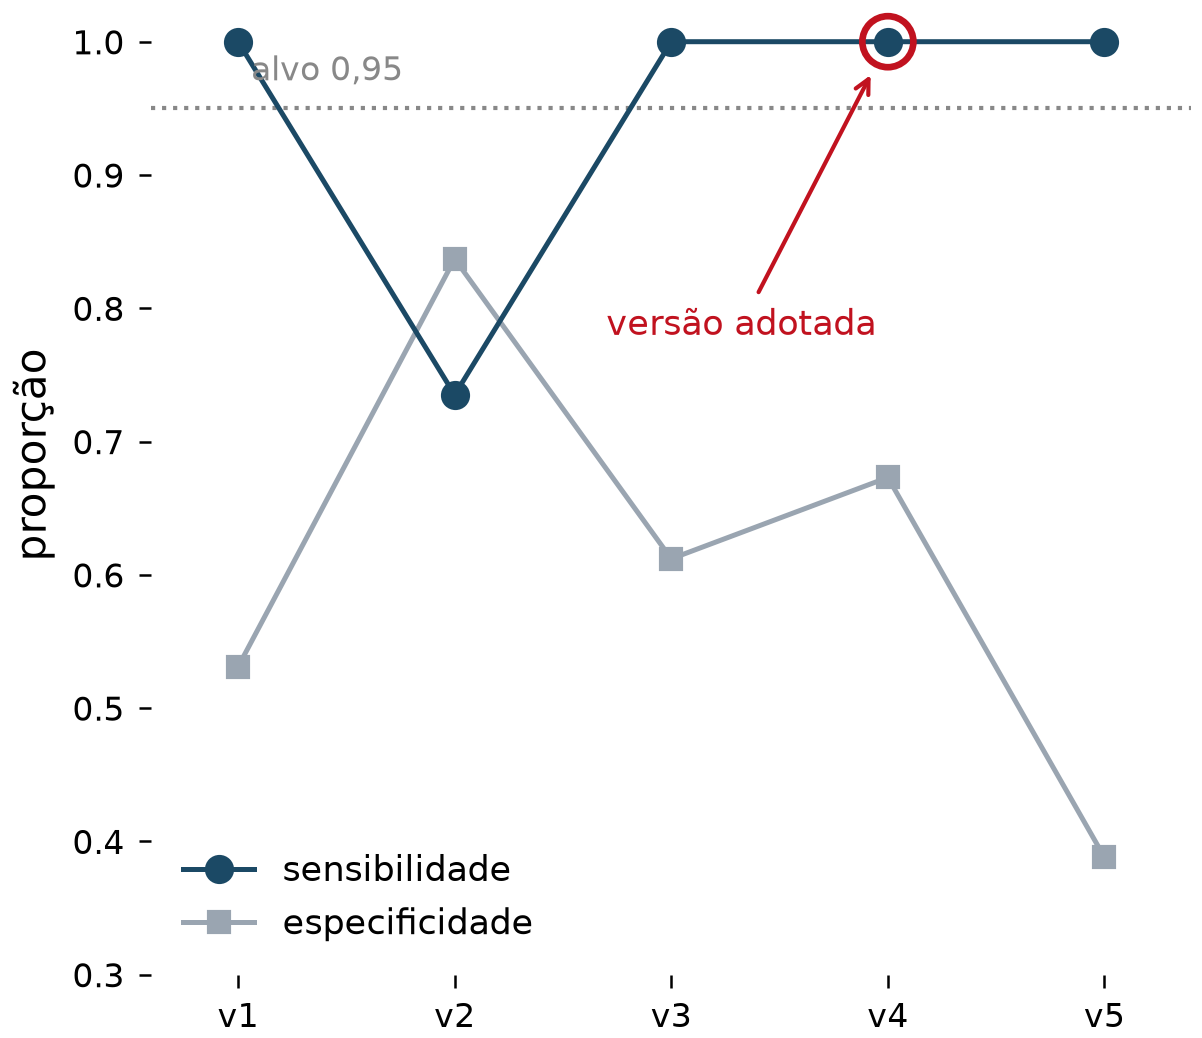
\includegraphics[width=0.80\linewidth]{Imagens/fig_calibracao.png}

        \par
        \raggedright
        \legend{Fonte: elaborada pelo autor.}
    \end{minipage}
\end{figure}

Adotou-se a quarta versão, que aprova as 49 obras e rejeita 67,3\% do ruído: entre as versões de sensibilidade 1,0, é a de maior especificidade. A assimetria é deliberada. Na triagem por título, excluir indevidamente é irreversível, porque o registro não volta a ser examinado, ao passo que incluir indevidamente custa apenas uma leitura a mais adiante.

Para efeito de reprodução, o classificador foi operado com o modelo Claude Opus, da Anthropic, em lotes de 250 registros, com saída estruturada e índice explícito por registro. Sem esse índice, o modelo perde a correspondência entre decisão e registro, defeito observado na aferição de custo. O enunciado adotado, as métricas das cinco versões e a decisão registrada para cada registro estão no repositório do projeto.

 

A triagem operou em dois passes. O primeiro decide apenas escopo, isto é, se o registro trata de algum dos eixos e guarda relação identificável com sistema de informação, dado ou especificação técnica. O segundo atribui grau de pertinência às questões de mapeamento, em quatro níveis: contribuição central, quando o artefato é o objeto declarado do trabalho; parcial, quando o aporte é secundário; tangencial; e não pertinente. Antes dos dois passes aplica-se um filtro determinístico de domínio alheio, que operacionaliza CE3 por marcadores léxicos inequívocos. Por ser determinístico, ele foi conferido contra o conjunto de aferição antes de valer: não derruba nenhuma das obras pertinentes. O volume que descarta consta da Seção \ref{sec:conducao}.

\subsection{Procedimento de extração}

De cada estudo incluído foram extraídos dois conjuntos de atributos, com funções metodológicas distintas. O primeiro é de caracterização e seleção: identificador persistente, metadados bibliográficos, questão de mapeamento principal e grau de pertinência. Esses atributos sustentam a caracterização do corpus da Seção \ref{sec:conducao} e definem, na Seção \ref{sec:relacionados}, quais estudos compõem a matriz comparativa. O segundo conjunto é de dimensões de comparação, codificadas apenas para os estudos admitidos na matriz. As dimensões são cinco: modelo semântico padronizado, barramento assíncrono exposto, perfil humano integrado ao contexto, governança e soberania instanciadas, e persistência segregada por natureza do dado. Cada uma recebeu uma entre três codificações: tratamento central e instanciado, quando a dimensão é objeto declarado da contribuição e o trabalho descreve mecanismo concreto que a realiza; tratamento parcial ou apenas declarativo; ou não abordado. Os símbolos correspondentes constam da Tabela \ref{tab:relacionados}. Essa codificação foi feita sobre o resumo de cada trabalho, recuperado pelo identificador persistente; nos casos em que o resumo não pôde ser obtido, a codificação apoiou-se em título, veículo e palavras-chave, e esses casos estão assinalados na própria tabela. Todos os passos, expressões e decisões foram registrados e estão disponíveis no repositório do projeto\footnote{\url{https://github.com/Alhexx/qualificacao}}, o que permite reexecutar o mapeamento de ponta a ponta.

\section{Condução e Caracterização do Corpus}
\label{sec:conducao}

As 39 expressões declararam 56.572 registros no Scopus e devolveram os mesmos 56.572, sem perda por teto de navegação em nenhuma delas. Somados os 1.589 registros do OpenAlex, chega-se a 58.161 registros brutos, que a Tabela \ref{tab:triagem} reduz por etapas.

Esses 58.161 são retornos, não trabalhos distintos: uma obra recuperada por três expressões aparece três vezes na contagem. A deduplicação resolve isso e remove 29,9\% do material, proporção que mede a sobreposição deliberada entre expressões vizinhas. Tomada cada base em separado, o Scopus responde por 39.646 registros distintos e o OpenAlex por 1.494, enquanto a união das duas produz 40.201. A soma das partes excede a união em 939, e essa diferença são os trabalhos que as duas bases recuperaram e que a união conta uma vez só; a contribuição exclusiva do OpenAlex fica, portanto, em 555 registros.

Sobre os 40.201 incidem os critérios eliminatórios. O filtro de tipo de documento descarta 1.656 registros por CE4, a janela temporal de CI5 descarta outros 26 e o filtro determinístico de domínio alheio retira 1.078. Restam 37.441 registros.

Antes da triagem, esse conjunto ainda perde o retorno de seis das 39 expressões de busca. Essas expressões foram executadas, mas, somadas, trazem cerca de treze mil registros que nenhuma outra expressão recupera, e entre eles há uma única obra do conjunto de controle. Deixá-las de fora reduz o conjunto de 37.441 para 24.314 registros e o recobrimento do conjunto de controle de 49 para 48 obras; os seis eixos continuam cobertos pelas expressões mais precisas de cada um.

O primeiro passe do classificador, a triagem por título, decide apenas se o registro está no escopo. Ele aprovou 17.985 dos 24.314 registros, sendo 15.267 por decisão de inclusão e 2.718 por dúvida, e reprovou 6.329. As 48 obras de controle presentes no conjunto foram todas aprovadas, o que confirma em escala real a sensibilidade medida na calibração sobre as 49 alcançadas pela busca.

O segundo passe atribui a cada um dos 17.985 aprovados um grau de pertinência às questões de mapeamento: contribuição central, parcial, tangencial ou não pertinente. Foram 1.942 registros de contribuição central e 5.345 de contribuição parcial, e o corpus incluído reúne esses dois graus, num total de 7.287 trabalhos. Os 10.698 restantes, tangenciais ou não pertinentes, ficam de fora. O ponto de corte, entre o grau parcial e o tangencial, foi fixado por medição: ele retém 44 das 48 obras de controle, e as quatro que ficam de fora são conceituais ou tangenciais, entre elas um levantamento de simulados de evacuação e uma discussão filosófica sobre centralidade humana em inteligência artificial \cite{taylor2023human}.

Por fim, resta saber quanto desse corpus depende da varredura temática no OpenAlex, que é a parte frágil do procedimento. Refazendo a contagem só com o que veio do Scopus, o corpus incluído passa de 7.287 para 6.887 trabalhos, e os de contribuição central, de 1.942 para 1.775. A base complementar responde por 5,5\% do corpus e por 8,6\% do seu núcleo, e o padrão descrito na Seção \ref{sec:relacionados} se sustenta sobre os 1.775 do Scopus como se sustentava sobre os 1.942. Pode-se afirmar, portanto, que o impacto da varredura sobre o resultado é baixo.

\begin{table}[htb]
\centering
\caption{Etapas de triagem e volumes resultantes}
\label{tab:triagem}
\scriptsize
\begin{tabularx}{\textwidth}{@{}X r@{}}
\toprule
\textbf{Etapa} & \textbf{Registros} \\
\midrule
Expressões de busca submetidas ao Scopus & 39 \\
Registros declarados pela base & 56.572 \\
Registros recuperados no Scopus & 56.572 \\
Registros recuperados no OpenAlex & 1.589 \\
\midrule
Total bruto & 58.161 \\
Únicos após deduplicação por identificador, DOI e título & 40.201 \\
Após filtro de tipo de documento (CE4) & 38.545 \\
Após janela temporal (CI5) & 38.519 \\
Após filtro determinístico de domínio alheio (CE3) & 37.441 \\
\midrule
Submetidos à triagem por título & 24.314 \\
Aprovados quanto ao escopo & 17.985 \\
Classificados como de contribuição parcial & 5.345 \\
Classificados como de contribuição central & 1.942 \\
\midrule
\textbf{Corpus incluído} & \textbf{7.287} \\
Conjunto comparativo após S1 e S2 & 822 \\
\bottomrule
\end{tabularx}
\legend{Fonte: elaborada pelo autor.}
\end{table}

\subsection{Recobrimento aferido}
\label{sec:recobrimento}

Uma busca automatizada só sustenta uma afirmação de ausência se tiver sido aferida. A aferição aqui segue a prática de confrontar a busca com um conjunto de obras pertinentes reunido por outro caminho, que \citeonline{zhang2011identifying} denominam \textit{quasi-gold standard}: obras identificadas antes da busca, por leitura do domínio e encadeamento de referências ao longo da pesquisa exploratória.

A composição desse conjunto obedece a uma regra declarada, e não à preferência do pesquisador. Entram as obras cujo objeto declarado pertence ao escopo do mapeamento, isto é, gêmeo digital urbano, plataforma de cidade inteligente, contexto e semântica urbana, perfil humano ou resposta a emergência, desde que indexadas com identificador persistente e dentro da janela temporal. Ficam de fora a fundamentação de engenharia de software transversal, sobre mensageria, conteinerização, microsserviços e bancos de série temporal, e os guias de condução de mapeamento sistemático \cite{petersen2015guidelines,barn2017conducting}. Essas obras não tratam do objeto do mapeamento, e uma busca bem delimitada não deve encontrá-las. Se entrassem na aferição, cada uma contaria como falha da busca, quando a ausência delas é justamente o resultado esperado. Elas entram no trabalho por inclusão dirigida declarada, mecanismo previsto no protocolo e recomendado por \citeonline{petersen2015guidelines}.

Das 78 obras reunidas, a regra mantém 64 na aferição, e a busca alcança 49 delas, um recobrimento de 76,6\%. As quinze restantes se explicam por quatro motivos: a falta do qualificador urbano, o domínio adjacente, a indexação irregular e o filtro de tipo de documento. Cinco são obras gerais, entre elas a formulação original do conceito de gêmeo digital \cite{grieves2016digital}, as revisões de maior circulação do campo \cite{barricelli2019survey,rasheed2020digital,vanderhorn2021digital} e um levantamento de \textit{middleware} sensível ao contexto social \cite{liang2015social}. Nenhuma expressão as alcança porque todas exigem o qualificador urbano, que é decisão deliberada do recorte, e por isso são ausências por construção, não por falha. Quatro estão em veículos de domínio adjacente, como pesquisa operacional, planejamento urbano, mobilidade e marketing, cujo vocabulário não cruza as facetas técnicas das expressões. Cinco estão fora da indexação regular do Scopus: três capítulos de livro ou periódicos de indexação irregular e duas obras apresentadas em conferências brasileiras. A última, uma nota editorial sobre a passagem da cidade inteligente ao gêmeo digital urbano \cite{yeh2024from}, foi alcançada pela busca e descartada pelo filtro de tipo de documento.

Por trás dessa leitura está uma distinção que convém deixar explícita: o corpus do mapeamento não coincide com a bibliografia deste trabalho. O mapeamento recupera o estado da arte do objeto, ao passo que a fundamentação tecnológica e metodológica chega por inclusão dirigida. Um protocolo que recuperasse por expressão temática um estudo comparativo de bancos de série temporal estaria mal delimitado, e não melhor calibrado.

A Figura \ref{fig:corpus} caracteriza os 7.287 trabalhos incluídos. A distribuição temporal mostra crescimento acelerado e recente, com mais da metade do corpus publicada de 2024 em diante, o que mostra um campo ainda em consolidação. A distribuição por questão de mapeamento concentra 3.009 trabalhos em QP1, contra 1.031 em QP3 e 1.018 em QP4, assimetria que mostra o campo concentrado na infraestrutura de interoperabilidade, e não em integrar o fator humano ou em instanciar governança. A assimetria, por si só, não estabelece a lacuna, uma vez que mil trabalhos em QP3 atestam a existência de pesquisa sobre o tema; o que ela indica é que o esforço se reparte entre frentes que raramente se encontram no mesmo artefato, observação que a matriz da Seção \ref{sec:relacionados} qualifica no nível do trabalho individual.

\begin{figure}[H]
	\centering
	\caption{Caracterização do corpus incluído}
	\label{fig:corpus}
	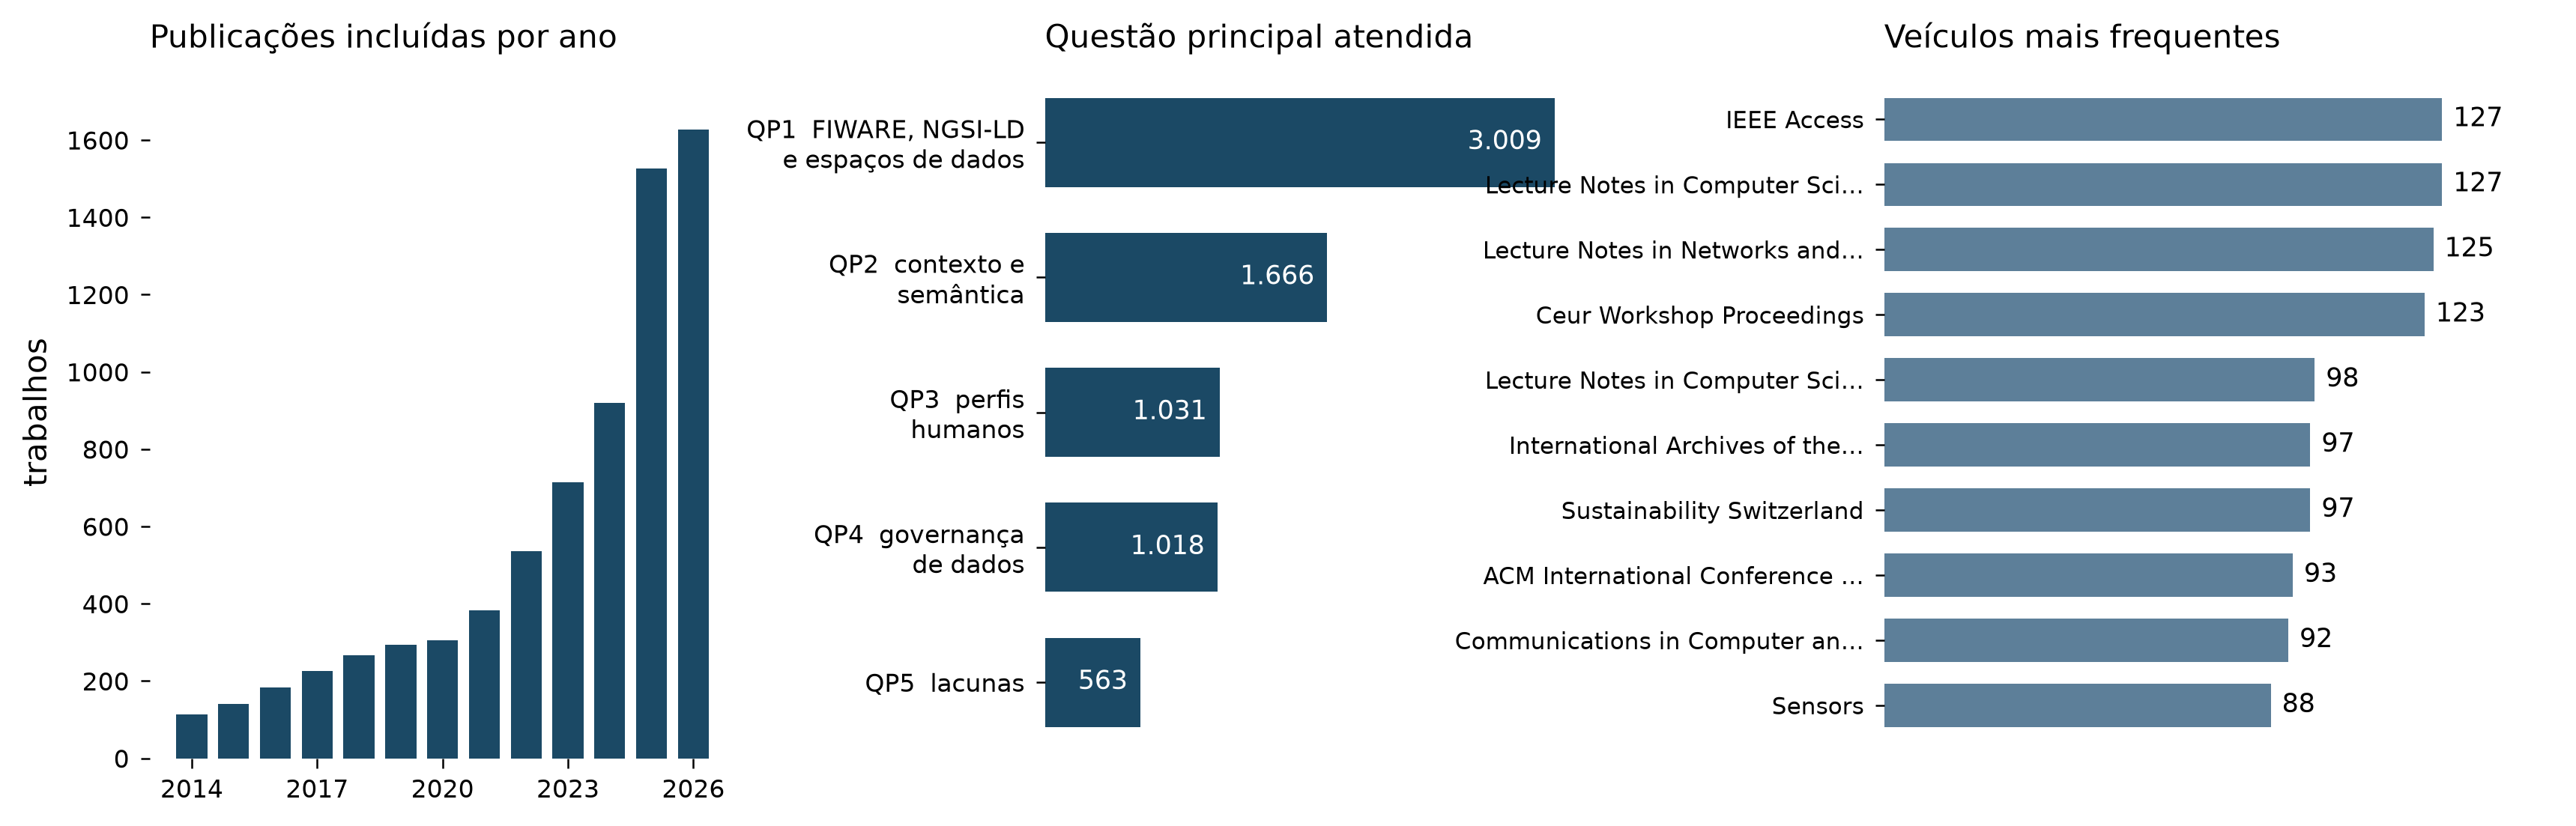
\includegraphics[width=\textwidth]{Imagens/fig_corpus.png}
	\legend{Fonte: elaborada pelo autor sobre os 7.287 trabalhos incluídos. A questão de mapeamento principal é atribuída na triagem de pertinência, descrita na Seção \ref{sec:procedimento-triagem}.}
\end{figure}

\section{Resultados por Questão de Mapeamento}
\label{sec:resultados-msl}

A QP1 pergunta como o FIWARE e os espaços de dados têm sido empregados na construção de gêmeos digitais urbanos e quais componentes se repetem nessas soluções. Para o FIWARE, a resposta é clara: o corpus o confirma como ecossistema de referência para plataformas urbanas abertas. Quando ele é levado a gêmeos digitais urbanos, como em \citeonline{bauer2021urban} e \citeonline{ditorrepadula2025smart} \cite{cirillo2019standard,bauer2022fiware,salhofer2019building}, repete-se o mesmo arranjo: o \textit{Context Broker}, uma camada de conexão a dispositivos e uma camada de persistência histórica. A ele se associam identidade e autorização. Somam-se a esses trabalhos plataformas municipais em operação. Entre elas estão o concentrador coreano de dados urbanos construído sobre padrões abertos \cite{jeong2020city} e a arquitetura de cidade baseada em conhecimento de \citeonline{badii2017analysis}. Na mesma linha, o arcabouço DUET interliga gêmeos digitais urbanos interoperáveis em escala europeia \cite{raes2022duet}. Nesse conjunto, o barramento de mensageria continua aparecendo como detalhe interno do broker, sem ser exposto como ponto de extensão, isto é, como lugar em que outros serviços possam se conectar ao fluxo de mudanças.

Para os espaços de dados, a resposta é menos coesa. A literatura se divide em duas frentes que pouco dialogam: uma trata dos modelos de referência e dos arranjos de governança, e a outra propõe a convergência entre espaços de dados e gêmeos digitais \cite{otto2019international,idsa2022ram,tardieu2022role,gaiax2022architecture,somma2023digital,uslander2022symbiotic,coppolino2025simulation,vogt2024towards}. No plano urbano, \citeonline{cuno2019data} são a referência mais direta. O trabalho de \citeonline{galij2025evaluating} é o único do corpus a quantificar a sobrecarga de desempenho da camada de soberania, e esse achado entrou como restrição de projeto na Seção \ref{sec:governanca}.

A QP2 pergunta que mecanismos de sensibilidade ao contexto e de raciocínio semântico as arquiteturas de gêmeos digitais urbanos reportam, e a resposta é a mais fragmentada. A literatura de \textit{middleware} sensível ao contexto é tecnicamente sofisticada \cite{lopes2009context,lopes2013middleware,liang2015social,sezer2018context}, mas antecede a consolidação do NGSI-LD e não dialoga com o vocabulário de gêmeos digitais. Já os trabalhos de gêmeos urbanos que discutem raciocínio tratam de simulação física, e não de raciocínio simbólico sobre os relacionamentos entre entidades. Os que mais se aproximam investigam como representar o NGSI-LD em RDF e consultá-lo em \textit{SPARQL Protocol and RDF Query Language} (SPARQL), as linguagens da Web Semântica para descrever e consultar grafos \cite{abid2022toward,viola2019mapping,drobnic2026automatic,gonzalez2024reshaping}. Eles demonstram que é viável percorrer o grafo de relacionamentos, mas tratam essa travessia como problema de consulta e não prescrevem como ligar o resultado a um fluxo que reage a eventos em tempo crítico. \citeonline{gao2017automated} descrevem a descoberta e a composição automatizadas de fluxos sobre dados urbanos semânticos, e \citeonline{bouloukakis2023enabling} constroem sobre NGSI uma camada de publicação e assinatura para sistemas de transporte. Os dois estreitam a distância entre raciocínio e resposta reativa, mas ficam no nível de um componente isolado, sem trazer perfil humano nem governança para o mesmo desenho. Em outra direção, \citeonline{austin2020architecting} combinam modelo semântico e aprendizado de máquina numa arquitetura de gêmeo digital urbano, e \citeonline{an2019global} propõem um adaptador semântico para a interoperação entre cidades.

A QP3 pergunta como os perfis humanos, com suas restrições de acessibilidade e vulnerabilidades, são representados e integrados ao modelo de contexto urbano. No domínio industrial, essa representação está madura \cite{asad2023human,okegbile2022edge}. No urbano, ainda é incipiente. O cidadão aparece como fonte de percepção e de participação \cite{luo2025perception,qanazi2025integrating}. A literatura também analisa de forma crítica a agência cidadã, isto é, o quanto ele de fato age sobre os sistemas que o envolvem \cite{tappert2024citizen,dejaeger2026right}. Só a literatura de evacuação e mobilidade trata restrição de acessibilidade como atributo que o sistema usa em cálculo \cite{hashemi2018emergency,deng2022semantic,allahbakhshi2026zuriact,wins2024enhancing}. Cada trabalho dessa linha, porém, usa um modelo de perfil próprio, sem integração a um modelo de contexto urbano padronizado. O precedente mais próximo está em \citeonline{liu2023urban}, que montam perfis de usuários móveis sobre um grafo de conhecimento urbano, embora para recomendar conteúdo e não para responder a emergências. \citeonline{zeng2025knowledge} oferecem um precedente de natureza análoga, combinando grafo de conhecimento e modelo oculto de Markov para personalização urbana, e \citeonline{rivadeneira2024confluence} propõem um modelo de integração que põe o humano no laço de decisão. Nenhum estudo do corpus, porém, representa o perfil humano como entidade NGSI-LD de primeira classe, ligada por relacionamentos às edificações e aos eventos no mesmo grafo.

A QP4 pergunta que estratégias de governança, soberania e proteção de dados as plataformas urbanas federadas adotam quando atributos pessoais sensíveis entram no processamento. A literatura concentra-se em três mecanismos: o conector como ponto único de aplicação de política, a identidade auto-soberana e a arquitetura corporativa de referência para efetivar a soberania digital \cite{idsa2022ram,gaiax2022architecture,sanchezserna2026data,firdausy2022towards}. Na identidade auto-soberana, o titular controla as próprias credenciais, sem depender de um provedor central. Soma-se a eles a identificação de vetores de exposição de perímetro, os pontos por onde um ataque pode atravessar a fronteira da plataforma \cite{perata2023security}. A literatura de gêmeos digitais urbanos, porém, raramente instancia esses mecanismos, e na maioria dos trabalhos a privacidade continua no plano das declarações de princípio. A análise de riscos de \citeonline{fontes2024human} é a exceção mais consistente. A ontologia de consentimento e contrato de \citeonline{kurteva2023smashhitcore} vai além, porque modela em vocabulário formal os elementos que a proteção de dados pessoais exige em dados de sensores. É o precedente mais próximo do tratamento de consentimento que a Seção \ref{sec:governanca} adota.

A QP5 pergunta que lacunas permanecem abertas na interseção dos eixos anteriores. A resposta sai das quatro questões anteriores, na forma de cinco lacunas que a Seção \ref{sec:requisitos} liga aos requisitos:

\begin{description}[leftmargin=1.6cm,style=nextline]
	\item[L1] Perfil humano fora do grafo de contexto. Quando existem, os perfis ficam em bases separadas do modelo de contexto urbano, e por isso não é possível partir de um evento, passar pela infraestrutura e chegar à pessoa afetada percorrendo relacionamentos.
	\item[L2] Barramento de eventos tratado como detalhe interno. O fluxo de mudanças de contexto raramente é exposto para que outros serviços o assinem, o que obriga integrações por consulta periódica e eleva a latência de resposta.
	\item[L3] Dissociação entre raciocínio semântico e ciclo reativo. Percorrer relacionamentos é tratado como problema de consulta, e não como etapa do fluxo assíncrono que decide a resposta em tempo crítico.
	\item[L4] Governança declarativa, não instanciada. Os mecanismos de soberania aparecem como requisito, mas raramente viram componentes arquiteturais auditáveis, e seu custo de desempenho quase nunca é medido.
	\item[L5] Persistência única para dois perfis de acesso. Consultas geoespaciais sobre o estado corrente e agregações sobre séries históricas convivem nos mesmos mecanismos de persistência, e raramente motivam separá-los de forma deliberada.
\end{description}

\section{Trabalhos Relacionados}
\label{sec:relacionados}

Comparar trabalhos lado a lado exige decidir antes quais entram na comparação, e essa decisão precisa de regra explícita, sob pena de a matriz refletir a composição da amostra em lugar do estado do campo. A regra parte dos 1.942 trabalhos de contribuição central e faz duas perguntas, nas quais o trabalho precisa passar. A primeira, S1 (escala da contribuição), é se ele propõe algo que se possa posicionar na matriz. Valem arquitetura, plataforma ou sistema completo, especificação normativa de arquitetura e componente que instancie tecnicamente ao menos uma das cinco dimensões de comparação. Revisões e estudos puramente empíricos ficam de fora, por não proporem artefato. A segunda, S2 (ancoragem urbana), é se o objeto declarado do trabalho é a cidade, a infraestrutura urbana ou os serviços públicos urbanos. Nenhuma das duas perguntas olha para as dimensões da matriz: S1 e S2 decidem quem entra pela escala e pelo domínio, e as dimensões decidem o que se observa em cada trabalho admitido. Essa independência faz a matriz produzir evidência, e não repetir o próprio critério de entrada.

As duas perguntas retêm 822 trabalhos, conjunto grande demais para leitura integral. A Tabela \ref{tab:relacionados} confronta 15 deles, também escolhidos por regra declarada. Entram todos os que tratam duas dimensões como centrais e todos os que tratam como central alguma das quatro dimensões menos estudadas: comunicação assíncrona, perfil humano, governança e persistência segregada. As vagas restantes vão aos de maior pontuação somada nas cinco colunas, com dois pontos por tratamento central e um por parcial. A codificação apoia-se no resumo de cada trabalho, recuperado pelo identificador persistente, e o único caso em que o resumo não pôde ser obtido está assinalado na tabela.

\begin{table}[htb]
\centering
\caption{Posicionamento comparativo dos trabalhos relacionados}
\label{tab:relacionados}
\scriptsize
\begin{tabular}{@{}p{4.1cm}p{4.6cm}ccccc@{}}
\toprule
\textbf{Trabalho} & \textbf{Foco principal} & \hdrv{Modelo\\semântico} & \hdrv{Barramento\\assíncrono} & \hdrv{Perfil\\humano} & \hdrv{Governança} & \hdrv{Persistência\\segregada} \\
\midrule
\citeonline{badii2017analysis} & Arquitetura de cidade baseada em conhecimento com APIs de serviço & $\bullet$ & $\circ$ & -- & $\circ$ & $\circ$ \\
\citeonline{gao2017automated} & Middleware de descoberta e composição semântica de fluxos urbanos & $\bullet$ & $\bullet$ & $\circ$ & -- & -- \\
\citeonline{cheng2018fogflow} & Arcabouço de computação em névoa para serviços IoT urbanos & $\circ$ & $\bullet$ & -- & -- & -- \\
\citeonline{souza2018geographic} & Middleware de camadas geográficas para dados urbanos & $\circ$ & -- & -- & -- & $\bullet$ \\
\citeonline{cuno2019data} & Espaço de dados urbanos para soberania sobre arquiteturas de referência & $\circ$ & -- & -- & $\bullet$ & -- \\
\citeonline{jeong2020city} & Plataforma coreana de dados urbanos baseada em modelo comum & $\bullet$ & $\circ$ & -- & $\circ$ & -- \\
\citeonline{bauer2021urban} & Gêmeo digital urbano baseado em FIWARE e NGSI-LD & $\bullet$ & $\circ$ & -- & -- & -- \\
\citeonline{pereira2022platform}\,$^{\dagger}$ & Plataforma de integração de dados heterogêneos para aplicações urbanas & $\circ$ & -- & -- & $\circ$ & $\circ$ \\
\citeonline{raes2022duet} & Arcabouço DUET de gêmeos digitais urbanos interoperáveis e confiáveis & $\circ$ & $\circ$ & $\circ$ & $\circ$ & -- \\
\citeonline{bouloukakis2023enabling} & Plataforma NGSI publish/subscribe para transporte público IoT & $\bullet$ & $\bullet$ & -- & -- & -- \\
\citeonline{kurteva2023smashhitcore} & Ontologia de consentimento e contratos para conformidade com GDPR & $\bullet$ & -- & $\circ$ & $\bullet$ & -- \\
\citeonline{liu2023urban} & Grafo de conhecimento urbano para perfilamento de usuários móveis & $\bullet$ & -- & $\bullet$ & -- & -- \\
\citeonline{gonzalez2024reshaping} & Enriquecimento semântico de dados urbanos com NGSI-LD & $\bullet$ & $\circ$ & $\circ$ & -- & -- \\
\citeonline{rivadeneira2024confluence} & Modelo de integração IoT com humano no laço e privacidade preservada & $\circ$ & -- & $\circ$ & $\bullet$ & -- \\
\citeonline{zeng2025knowledge} & Grafo de conhecimento e modelo oculto de Markov para rotas personalizadas & $\bullet$ & -- & $\bullet$ & -- & -- \\
\midrule
\textbf{Proposta desta pesquisa} & Backend sensível ao contexto para gêmeo digital urbano & $\bullet$ & $\bullet$ & $\bullet$ & $\bullet$ & $\bullet$ \\
\bottomrule
\end{tabular}
\par\vspace{4pt}
\legend{Fonte: elaborada pelo autor. $\bullet$ tratamento central; $\circ$ tratamento parcial; -- não abordado. $^{\dagger}$ codificação apoiada em título, veículo e palavras-chave, por indisponibilidade do resumo.}
\end{table}

A coluna de semântica é a mais ocupada: entre os 15, são 9 tratamentos centrais e 6 parciais, e nenhum trabalho a ignora por completo. Isso reflete a maturidade que as plataformas urbanas abertas já consolidaram nesse eixo. As outras quatro colunas estão bem mais vazias. Comunicação assíncrona registra 3 tratamentos centrais, governança 3, perfil humano 2 e persistência segregada apenas 1, contra 12 trabalhos que não a abordam.

Nenhum dos 15 trabalhos trata como central mais de duas das cinco dimensões, e cinco chegam a duas. \citeonline{gao2017automated} e \citeonline{bouloukakis2023enabling} combinam modelo semântico e comunicação assíncrona, \citeonline{liu2023urban} e \citeonline{zeng2025knowledge} combinam modelo semântico e perfil humano, e \citeonline{kurteva2023smashhitcore} combina modelo semântico e governança. Nos cinco casos, o modelo semântico é a base à qual o trabalho acrescenta uma segunda capacidade, e nenhum chega a uma terceira.

Como a escolha dos 15 olhou para as dimensões, o teto de duas precisa ser conferido fora deles. Ele se mantém: nenhum dos 822 trabalhos que passam em S1 e S2 reúne indício de mais de duas dimensões. A matriz apenas torna esse teto legível trabalho a trabalho.

A ausência não é de capacidade, e sim de integração. As cinco capacidades existem e foram validadas isoladamente, ora em outro domínio, ora em outra escala, ora como componente isolado dentro do domínio urbano: perfilamento sobre grafo urbano \cite{liu2023urban,zeng2025knowledge}, consentimento formalizado em ontologia \cite{kurteva2023smashhitcore}, publicação e assinatura sobre NGSI \cite{bouloukakis2023enabling}, soberania em dados urbanos \cite{cuno2019data} e persistência segregada por natureza do dado \cite{souza2018geographic}. Não se encontrou um artefato arquitetural urbano que as reúna num mesmo desenho, contraste que a última linha da Tabela \ref{tab:relacionados} torna visível.

\section{Ameaças à Validade do Mapeamento}
\label{sec:ameacas-msl}

Cinco ameaças merecem registro, com o que foi feito para conter cada uma.

A primeira é a cobertura da base. O Scopus contempla periódicos e anais de conferência publicados pelas editoras que concentram a produção do campo, mas sua indexação, feita sob critério editorial, não é exaustiva, e a aferição contra o conjunto de referência localizou cinco obras pertinentes fora de sua indexação. Três delas foram recuperadas pelo nome no OpenAlex. O risco residual é o de obras pertinentes fora das duas bases; replicar as expressões em IEEE Xplore e ACM Digital Library fica registrado como extensão natural do protocolo.

A segunda é a diferença de regime entre as duas bases. A busca no Scopus é exaustiva em relação a cada expressão, ao passo que a varredura no OpenAlex retornou uma amostra por relevância, porque aquela interface não oferece busca restrita a campo nem deixa percorrer o retorno inteiro. Três providências contêm o efeito: a diferença está declarada na Seção \ref{sec:protocolo}, a contribuição de cada base é separável registro a registro, e a Seção \ref{sec:conducao} mostra que descartar tudo o que veio da varredura reduz o corpus em 5,5\% sem alterar o padrão encontrado. Dois dos quinze trabalhos da matriz chegaram por esse caminho, entre eles o precedente de consentimento discutido na Seção \ref{sec:governanca}; eles permanecem no confronto por inclusão dirigida declarada, e não por recuperação sistemática. O risco residual é que a varredura tenha deixado passar trabalhos que só ela alcançaria, e esse risco não tem como ser medido pelo interior do próprio procedimento.

A terceira é a triagem assistida por modelo de linguagem. O erro desse procedimento é sistemático, não aleatório: um enunciado mal formulado erra da mesma forma em todos os registros. Por isso o enunciado foi aferido antes da aplicação, contra 49 obras pertinentes e contra 49 registros de ruído, e só foi adotado após aprovar as 49 (Figura \ref{fig:calibracao}); o enunciado e cada decisão individual foram registrados, o que torna a triagem reexecutável e auditável por amostragem. Restam dois limites: a especificidade de 67,3\% admite falsos positivos no conjunto incluído, que a etapa de seleção posterior filtra; e a sensibilidade de 1,0 foi aferida sobre o conjunto de referência, e vale para ele.

A quarta é a triagem feita sobre título, veículo e ano, já que a base primária não devolve o resumo. Um trabalho cujo título não anuncia o mecanismo pode ter sido subestimado na atribuição de pertinência. Na matriz comparativa, em que essa limitação pesaria mais, a codificação foi refeita sobre o resumo de cada trabalho, recuperado pelo identificador persistente; o único caso em que isso não foi possível está assinalado na Tabela \ref{tab:relacionados}.

A quinta é o revisor único, sem aferição de concordância entre avaliadores. A contenção foi tornar cada decisão verificável: critérios explícitos, regra de seleção da matriz declarada antes da codificação, regra de composição do conjunto de aferição declarada antes da medida, e o registro integral de expressões, retornos e decisões no repositório do projeto. Isso não substitui um segundo revisor, mas permite que qualquer leitor refaça o caminho e aponte onde discorda. O conjunto de aferição foi reunido pelo mesmo pesquisador e reflete, por isso, o recorte de leitura dele. É um \textit{quasi}-gold standard, e não um padrão-ouro, de modo que a sensibilidade medida vale em relação a esse conjunto e não à literatura inteira.

Especificações e documentos de arquitetura de referência evoluem por versões, e a caracterização aqui apresentada refere-se às versões consultadas, com registro de data de acesso nas referências correspondentes.

	\chapter{Arquitetura Proposta}
\label{cap:arquitetura}

Este capítulo descreve a arquitetura de \textit{backend} concebida para suprir as lacunas consolidadas na Seção \ref{sec:resultados-msl}. A exposição parte dos requisitos e da lacuna que origina cada um, registra as decisões estruturantes, descreve as camadas lógicas, a modelagem semântica das entidades e os componentes que constituem a contribuição deste trabalho, e encerra com um cenário de missão crítica.

\section{Visão Geral e Princípios de Projeto}
\label{sec:visao-geral}

A arquitetura organiza-se em cinco camadas lógicas em torno de um núcleo semântico único, seguindo um modelo de referência de gêmeos digitais urbanos em cinco camadas. A Figura \ref{fig:arquitetura} apresenta a organização resultante, com os macro componentes e as interfaces de dados entre eles, isto é, o que cada componente consome e fornece. As setas rotulam essas interfaces e não a sequência de um caso de uso particular, que varia conforme o cenário e aparece na Seção \ref{sec:cenario}.

\begin{figure}[!htbp]
    \centering

    \begin{minipage}{0.80\textwidth}
        
        \caption{Macrocomponentes da arquitetura proposta, por camada}
        \label{fig:arquitetura}
        \centering
        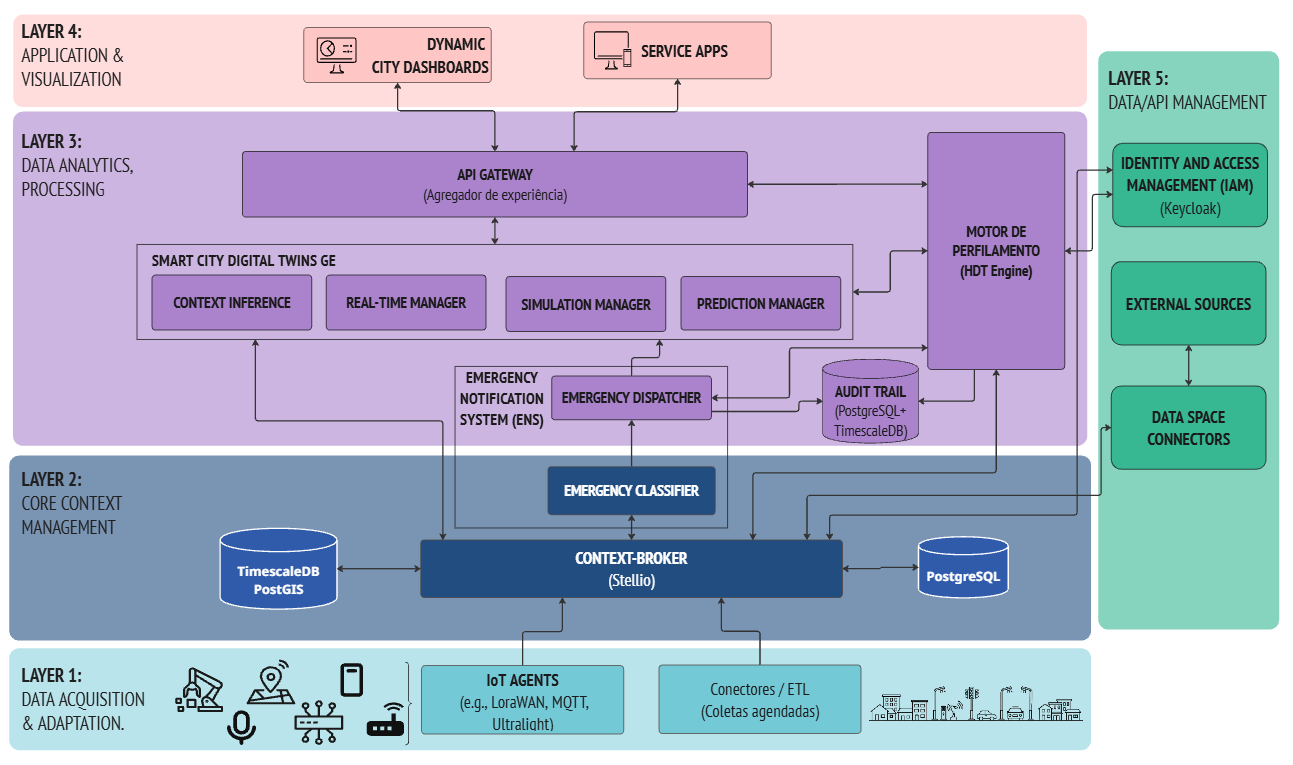
\includegraphics[width=\linewidth]{Imagens/fig_arquitetura.png}

        \par
        \raggedright
        \footnotesize
        \legend{Fonte: elaborada pelo autor sobre o modelo de referência em cinco camadas.}
    \end{minipage}
\end{figure}

Cinco princípios derivados das lacunas do mapeamento governam o desenho: fonte única de verdade, integração assíncrona, separação entre representação e política, persistência especializada e componente trocável fora do contêiner que o usa. O contexto urbano tem fonte única de verdade, de modo que infraestrutura, evento e pessoa são entidades NGSI-LD no \textit{Context Broker} e nenhum serviço mantém representação paralela desse estado. A integração entre o núcleo e os componentes de aplicação é assíncrona e declarativa. A representação está separada da política, com o modelo semântico descrevendo o que existe e os componentes de domínio o que fazer. A persistência é especializada por perfil de acesso. Por fim, componente que se pretenda trocável fica externo ao contêiner que o utiliza, critério que explica por que o Motor de Perfilamento e o \textit{Emergency Notification System} não residem dentro do bloco de processamento de contexto.

\section{Requisitos e Rastreabilidade}
\label{sec:requisitos}

A Tabela \ref{tab:requisitos} enuncia os requisitos funcionais (RF) e não funcionais (RNF), cada um com indicação da lacuna que o motiva. Com essa rastreabilidade, a avaliação do Capítulo \ref{cap:avaliacao} verifica atendimento de requisito, em vez de aferir desempenho de forma genérica.

O limiar de RNF1, de 1~s no percentil 95 e 2~s no percentil 99 (Tabela \ref{tab:requisitos}), é uma meta de projeto, e não um valor normativo: nenhuma norma encontrada define a latência de um \textit{backend} de notificação personalizada. A referência mais próxima é o prazo de 4~s que a 3GPP TS 22.268 fixa para a entrega ao terminal da notificação primária de alerta de terremoto e tsunami, que não inclui o \textit{backend} \cite{etsi2026ts122268}. Atribui-se ao \textit{backend} metade desse prazo, de modo que a cadeia completa fique em até 6~s no pior caso. Sistemas de alerta urbano medem, em trechos distintos do de RNF1, de dezenas a centenas de milissegundos \cite{maltezos2022smart,zhang2025developing}, o que deixa margem para a travessia de grafo e as regras.

\begin{table}[H]
\centering
\caption{Requisitos funcionais e não funcionais, com a lacuna de origem}
\label{tab:requisitos}
\scriptsize
\begin{tabularx}{\textwidth}{@{}l X l@{}}
\toprule
\textbf{Código} & \textbf{Requisito} & \textbf{Lacuna} \\
\midrule
RF1 & Ingerir dados de contexto em conformidade com NGSI-LD, validando o \texttt{@context} declarado e rejeitando \textit{payloads} semanticamente inconsistentes. & L1, L3 \\
RF2 & Representar o perfil do cidadão como entidade NGSI-LD de primeira classe, com relacionamentos navegáveis para entidades de infraestrutura e de evento. & L1 \\
RF3 & Registrar toda mudança de estado de contexto em um \textit{log} durável e ordenado, recuperável para reprocessamento. & L2 \\
RF4 & Admitir o registro de assinaturas declarativas que disparem notificação quando critérios de atributo, geografia ou relacionamento sejam satisfeitos, com endereço de notificação declarado pelo próprio assinante. & L2, L3 \\
RF5 & Derivar, a partir de um evento crítico, os destinatários da resposta, afetados e atuantes, por travessia de grafo combinada a predicado geoespacial e a critério de atributo. & L1, L3 \\
RF6 & Avaliar regras de personalização sobre o conjunto derivado e emitir resposta diferenciada por perfil, incluindo rota de evacuação compatível com as restrições declaradas e instrução de atuação a quem tem competência verificada. & L3 \\
RF7 & Consolidar telemetria de uso e atributos declarados em atualizações incrementais da entidade de perfil, com registro de proveniência por atributo. & L1 \\
RF8 & Materializar o estado corrente georreferenciado e o histórico de atributos em mecanismos de persistência distintos. & L5 \\
RF9 & Condicionar o acesso a atributos de perfil à autorização do núcleo semântico integrada ao serviço de identidade, registrando em trilha de auditoria a finalidade declarada e a decisão tomada. & L4 \\
RF10 & Expor aos clientes contratos agregados por caso de uso, com o recorte de contexto personalizado por pessoa, ocultando a topologia interna de serviços. & L2 \\
\midrule
RNF1 & Latência fim-a-fim entre a ingestão do evento crítico e a emissão da notificação personalizada, em até 1~s no percentil 95 e em até 2~s no percentil 99. & L2, L3 \\
RNF2 & Durabilidade das mensagens de contexto, sem perda de eventos críticos sob pico de carga. & L2 \\
RNF3 & Escalabilidade horizontal independente por serviço, sem reimplantação do núcleo semântico. & L2 \\
RNF4 & Tolerância à indisponibilidade de consumidores não críticos, sem interrupção da ingestão. & L2 \\
RNF5 & Minimização dos dados pessoais processados, restringindo a propagação de atributos sensíveis ao estritamente necessário à decisão. & L4 \\
RNF6 & Explicabilidade da decisão de personalização, com registro da regra aplicada e dos atributos considerados. & L4 \\
RNF7 & Reprodutibilidade integral do ambiente por infraestrutura declarada como código. & L5 \\
RNF8 & Extensibilidade do modelo semântico a novos domínios sem alteração dos serviços existentes. & L1 \\
\bottomrule
\end{tabularx}
\legend{Fonte: elaborada pelo autor.}
\end{table}

\section{Decisões Arquiteturais}
\label{sec:adr}

As sete decisões estruturantes, designadas DA1 a DA7, seguem uma ordem de dependência, e cada uma delimita o espaço de escolha da seguinte. São registradas segundo a prática de registro de decisão arquitetural recomendada por \citeonline{bass2021software}: o problema que resolvem, as alternativas consideradas, a escolha e a consequência aceita. Quando a justificativa é raciocínio de projeto, e não evidência, o texto o declara. DA1, DA2 e DA7 são detalhadas em texto, e DA3 a DA6 constam das Tabelas \ref{tab:adr} e \ref{tab:adr2}.

\subsection{Modelo de informação e interface de contexto (DA1)}

O modelo de informação precisa dar três coisas ao fluxo que leva um evento urbano à pessoa afetada: relacionamentos entre cidadão, edificação e evento que se possam percorrer (RF5), assinatura de mudanças por atributo, geografia ou relacionamento (RF4) e um vocabulário que um domínio novo estenda sem alterar os serviços existentes (RNF8). Esses requisitos vêm das lacunas L1 a L3 (Seção \ref{sec:resultados-msl}).

Três alternativas foram consideradas: o NGSI-v2, o NGSI-LD e uma API REST própria por domínio. O NGSI-v2 liga entidades só por convenção de nome (Seção \ref{sec:contexto}), e por isso a travessia (RF5) e a extensão do vocabulário (RNF8) ficam a cargo de cada aplicação. A API própria teria de construir as assinaturas (RF4) e exigiria alterar os serviços existentes a cada domínio novo (RNF8). O NGSI-LD atende aos três na mesma interface: trata relacionamentos como parte do modelo, especifica as assinaturas e declara o vocabulário no \texttt{@context}, que um domínio novo estende sem alterar os demais \cite{etsi2024ngsild}.

Portanto, depois dessa análise, o NGSI-LD foi adotado. Como o JSON-LD é uma serialização do RDF, o NGSI-LD mantém a base semântica do grafo sem exigir banco RDF nem SPARQL \cite{fiware2026catalogue,abid2022toward}. O custo é a complexidade: é preciso entender JSON-LD \cite{fiware2026tutorials}, e a interface fica presa à versão da especificação, hoje a TS 104 175 da ETSI \cite{etsi2026ts104175}.

\subsection{Implementação do \textit{Context Broker} (DA2)}

Adotado o NGSI-LD, resta escolher quem o implementa. O pré-requisito é oferecer os recursos de DA1, e quatro critérios da Seção \ref{sec:requisitos} comparam as candidatas: o registro durável das mudanças (RF3, RNF2), a escalabilidade por serviço (RNF3, estendida por raciocínio de projeto aos serviços internos do broker), a autenticação e a autorização nativas (RF9) e a latência fim a fim (RNF1), da qual o broker responde por uma parcela. Um quinto critério é de projeto: a coerência da persistência com DA4.

O catálogo do FIWARE lista três implementações com NGSI-LD \cite{fiware2026catalogue}, comparadas na Tabela \ref{tab:brokers} a partir da documentação de cada projeto e de duas avaliações de desempenho \cite{ntallaris2024benchmarking,lazidis2022publish}.

\begin{table}[!tp]
\centering
\caption{Implementações NGSI-LD de \textit{Context Broker} consideradas}
\label{tab:brokers}
\scriptsize
\begin{tabularx}{\textwidth}{@{}>{\raggedright\arraybackslash}p{2.5cm}>{\raggedright\arraybackslash}X>{\raggedright\arraybackslash}X>{\raggedright\arraybackslash}X@{}}
\toprule
\textbf{Atributo} & \textbf{Orion-LD} & \textbf{Scorpio} & \textbf{Stellio} \\
\midrule
Arquitetura & Processo único, em C/C++. & Microsserviços em Java, sobre \textit{Spring Cloud} e, em versão recente, \textit{Quarkus}. & Microsserviços em Kotlin, sobre \textit{Spring Boot} e \textit{Spring Cloud}. \\
\addlinespace
Cobertura da API NGSI-LD & Subconjunto dos \textit{endpoints}, segundo o catálogo; conformidade quase total com a versão 1.6.1, segundo o projeto. & Interface temporal opcional. & Interfaces de núcleo, temporal e de assinatura, em serviços distintos. \\
\addlinespace
Barramento interno & Sem barramento entre serviços; consumidor Kafka opcional para ingestão. & Kafka entre os serviços. & Kafka entre os serviços, com um evento por operação, publicado após o \textit{commit}. \\
\addlinespace
Persistência & MongoDB; histórico opcional em PostgreSQL com PostGIS e TimescaleDB. & PostgreSQL com PostGIS, inclusive nas consultas temporais \cite{ntallaris2024benchmarking}. & PostgreSQL com as extensões Timescale e PostGIS. \\
\addlinespace
Autenticação e autorização & Sem OAuth2 nativo \cite{lazidis2022publish}. & OAuth2 para autenticação e autorização \cite{lazidis2022publish,scorpio2026docs}; modelo de permissão não detalhado. & Nativas e opcionais, por OpenID Connect e OAuth2, validadas com Keycloak; permissão por entidade, tipo e escopo. \\
\addlinespace
\textit{Context Sources} e operação distribuída & Registro de \textit{Context Sources} e operações distribuídas, segundo o projeto. & Implantação centralizada, distribuída ou federada; fontes de contexto podem ser outros brokers. & Registro de \textit{Context Sources} e recuperação de entidades relacionadas nelas; operação distribuída em desenvolvimento. \\
\bottomrule
\end{tabularx}
\legend{Fonte: elaborada pelo autor, a partir de \cite{fiware2026catalogue,fiware2026orionld,scorpio2026docs,stellio2025docs}.}
\end{table}

O Orion-LD sai da comparação por três motivos: o registro durável, a escalabilidade e a persistência. O processo único não tem barramento entre serviços, e a tolerância a falhas exige um escalonador e um \textit{cluster} de brokers e de MongoDB \cite{ntallaris2024benchmarking}; por raciocínio de projeto, o \textit{log} de RF3 teria de ser montado fora do broker, e a escala só viria por réplica do processo inteiro. No Stellio, o serviço de busca publica cada evento no Kafka depois do \textit{commit} e na ordem do \textit{commit} \cite{stellio2025docs}. Sob carga alta, as arquiteturas em microsserviços escalam melhor que o Orion-LD \cite{ntallaris2024benchmarking}. Na persistência, o Orion-LD guarda o estado corrente em MongoDB e o histórico em PostgreSQL, dois motores de famílias distintas, enquanto DA4 fixa PostgreSQL com PostGIS e TimescaleDB. O critério de latência favorece o Orion-LD, mas prevalecem o registro durável e a escalabilidade, porque, por raciocínio de projeto, um alerta perdido custa mais do que centenas de milissegundos.

Entre Scorpio e Stellio, o pré-requisito e a escalabilidade não separam as candidatas: ambas são microsserviços ligados por Kafka, guardam o estado corrente em PostgreSQL com PostGIS e respondem de forma semelhante sob carga crescente \cite{ntallaris2024benchmarking,lazidis2022publish}, e \citeonline{lazidis2022publish} consideram o Scorpio o mais completo em funcionalidade. A decisão repousa em duas razões de alinhamento, a persistência e a identidade, e em uma razão prática, nenhuma medida neste trabalho. Na persistência, o Stellio guarda o histórico em TimescaleDB e o estado corrente em PostGIS, a combinação de DA4, enquanto no Scorpio todas as consultas do \textit{benchmark} rodaram em PostGIS; nesse \textit{benchmark}, o Stellio foi mais robusto na consulta temporal mais custosa, indício indireto, e não prova \cite{ntallaris2024benchmarking}. Na identidade, os dois usam OAuth2 \cite{lazidis2022publish}, mas só o Stellio documenta permissões por entidade, tipo e escopo, validadas com Keycloak \cite{stellio2025docs}. A razão prática, a familiaridade do autor com o Spring, pesa menos, porque o Spring também está na base de uma versão do Scorpio. O Stellio registra \textit{Context Sources} \cite{stellio2025docs}, recurso de que DA5 depende, e o encaminhamento das demais operações será testado na versão instalada.

Adota-se o Stellio \cite{stellio2025docs} com a opção \texttt{fail}. As consequências aceitas são cinco: o custo de implantação, a rejeição de escritas com o Kafka indisponível, o risco de latência, a reversibilidade parcial e a ausência de suporte a NGSI-v1 e NGSI-v2 \cite{fiware2026catalogue}. A pilha mínima inclui o barramento interno e um PostgreSQL com dois bancos. A opção \texttt{fail} troca disponibilidade da ingestão por consistência do registro: com uma única réplica do Kafka, como na prova de conceito, a indisponibilidade detectada vira escrita rejeitada, e a saída para produção é replicar o barramento, e não relaxar a opção. O risco de latência vem das avaliações, em que o Orion-LD ingeriu mais rápido por lote \cite{ntallaris2024benchmarking} e respondeu mais rápido em publicação e assinatura \cite{lazidis2022publish}, e a decisão deve ser revista se a latência medida no Capítulo \ref{cap:avaliacao} não couber em RNF1. A reversibilidade é parcial: trocar de broker altera a implantação, a integração com o Keycloak e o modelo de permissões de DA7, mas não os consumidores NGSI-LD, salvo diferenças de versão e cobertura. O Motor de Perfilamento e o \textit{Emergency Notification System} não leem o Kafka e se acoplam ao broker só pela assinatura NGSI-LD, embora dependam dele indiretamente, porque é por ele que o serviço de assinaturas recebe as mudanças que disparam as notificações \cite{stellio2025docs}.

\subsection{Integração, persistência, contexto derivado e regras (DA3 a DA6)}

A Tabela \ref{tab:adr} reúne DA3 e DA4, e a Tabela \ref{tab:adr2}, DA5 e DA6.

\begin{table}[H]
\centering
\caption{Decisões arquiteturais sobre a integração por assinatura e a persistência}
\label{tab:adr}
\scriptsize
\begin{tabularx}{\textwidth}{@{}l>{\raggedright\arraybackslash}p{3.1cm}XX@{}}
\toprule
\textbf{Código} & \textbf{Problema e decisão} & \textbf{Alternativas descartadas} & \textbf{Consequência aceita} \\
\midrule
DA3 & Definir como os componentes de domínio tomam conhecimento das mudanças de contexto (RNF2, RNF4). Adota-se a assinatura NGSI-LD como integrador primário, com endereço de notificação declarado por cada assinante. & Consumo direto do barramento interno do broker, que exigiria montar o evento no formato interno da implementação e criaria acoplamento de versão; consulta periódica ao broker, incompatível com RNF1. & Consistência eventual entre o núcleo e as visões derivadas, exigindo que as consultas tolerem defasagem limitada. \\
\addlinespace
DA4 & Atender consulta geoespacial sobre estado corrente e agregação sobre série histórica, de requisitos de indexação incompatíveis (RF8, RNF3). Adota-se a persistência que o próprio núcleo opera, PostgreSQL com PostGIS \cite{obe2021postgis} e TimescaleDB \cite{timescale2025docs}, escolha corroborada empiricamente \cite{john2023application,rudakov2023comparison,simanjuntak2022multiple}. A trilha de auditoria de RF9 usa uma instância própria do mesmo motor (DA7). & Persistência unificada de propósito geral, pela degradação previsível de um dos perfis; banco de séries temporais isolado, pela ausência de predicados geométricos; réplica do contexto em bases próprias dos componentes, por contrariar a fonte única de verdade; banco de documentos para a trilha, por introduzir um terceiro paradigma de persistência no capítulo em que a persistência excluiu um concorrente (DA2). & Os componentes de domínio passam a depender do desempenho de consulta do núcleo, que se torna objeto de medição no Capítulo \ref{cap:avaliacao}, e as consultas temporais custam caro em todos os brokers avaliados \cite{ntallaris2024benchmarking}. \\
\bottomrule
\end{tabularx}
\legend{Fonte: elaborada pelo autor.}
\end{table}

\begin{table}[H]
\centering
\caption{Decisões arquiteturais sobre o contexto derivado e a derivação da resposta}
\label{tab:adr2}
\scriptsize
\begin{tabularx}{\textwidth}{@{}l>{\raggedright\arraybackslash}p{3.1cm}XX@{}}
\toprule
\textbf{Código} & \textbf{Problema e decisão} & \textbf{Alternativas descartadas} & \textbf{Consequência aceita} \\
\midrule
DA5 & Entregar o contexto derivado pelos gestores sem expor a topologia interna do bloco. Registra-se o bloco no broker como \textit{Context Source} NGSI-LD \cite{etsi2024ngsild}. & Expor o bloco só por ligações diretas, sem registro no broker, o que multiplicaria interfaces e deixaria o contexto derivado invisível a quem consulta apenas o broker. & A consulta encaminhada é síncrona, logo gestor cujo cálculo não cabe no tempo da requisição precisa pré-computar e publicar o resultado como entidade. \\
\addlinespace
DA6 & Derivar a resposta personalizada de forma auditável (RNF6). Adota-se, nesta etapa, motor de regras determinístico e explicável sobre o grafo semântico, exigência derivada da lacuna L4 e dos riscos de discriminação por perfil inferido \cite{fontes2024human}. & Modelo estatístico opaco, que não permitiria registrar a regra aplicada e os atributos considerados em cada decisão; arranjos híbridos \cite{lex2025hybrid} ficam como evolução posterior, sem ruptura arquitetural. & Menor capacidade de generalização para padrões não antecipados na especificação das regras. \\
\bottomrule
\end{tabularx}
\legend{Fonte: elaborada pelo autor.}
\end{table}

A consequência de DA3 merece uma explicação além da tabela. Pela assinatura, o núcleo avisa cada assinante quando um dado muda, sem que um componente precise conhecer os outros \cite{eugster2003many}. O aviso chega um instante depois da mudança, e nesse intervalo um componente pode usar um dado já desatualizado, o que a literatura chama de consistência eventual \cite{kleppmann2017designing}. O barramento interno do broker serve para guardar os eventos e escalar a ingestão; nenhum componente deste trabalho lê os tópicos dele.

RF3 pede um registro durável, ordenado e recuperável. Durável quer dizer que um evento confirmado não se perde: o Kafka só o confirma depois de copiá-lo para as réplicas, se o produtor exigir isso, e com uma única réplica, como na prova de conceito, a proteção se limita ao disco do barramento. Ordenado quer dizer que os eventos são lidos na ordem de gravação, mas só dentro de cada partição, e a documentação consultada não informa como o Stellio os distribui; por isso nenhuma regra deste trabalho depende da ordem entre eventos de origens diferentes. Recuperável quer dizer que um consumidor parado retoma de onde parou, dentro da janela de retenção, e como os últimos eventos podem chegar duas vezes, processá-los de novo não pode alterar o resultado. A documentação consultada não descreve essa política no serviço de assinaturas do Stellio; nos consumidores da camada de orquestração, ela é decisão de projeto.

Restam dois modos de perda: o evento que nunca chega ao Kafka e a notificação que nunca chega ao assinante. No primeiro, a escrita é aceita e o evento se perde, porque o barramento fica fora do ar por mais tempo do que o produtor tenta publicar ou porque a fila do produtor se esgota \cite{stellio2025docs}. A opção \texttt{fail} de DA2 estreita esse caminho: detectada a indisponibilidade, as escritas passam a ser rejeitadas, e o risco residual se limita às aceitas pouco antes da detecção \cite{stellio2025docs}. No segundo, o evento chega ao tópico, mas a notificação não chega ao assinante, por falha no envio ou no processamento interno do serviço de assinaturas. A especificação registra a falha de envio na própria assinatura \cite{etsi2024ngsild}, e a documentação consultada do Stellio não descreve reenvio. Por raciocínio de projeto, a entrega ao assinante nesse modo é tratada, então, como de no máximo uma vez. Para consumidor não crítico isso basta, e RNF4 o admite. Para o despacho de emergência não basta, e a Tabela \ref{tab:falhas} reúne os três mecanismos que cobrem o caminho, cada um num trecho distinto.

\begin{table}[!htbp]
\centering
\caption{Tratamento de falha ao longo do caminho de uma mudança de contexto}
\label{tab:falhas}
\scriptsize
\begin{tabularx}{\textwidth}{@{}>{\raggedright\arraybackslash}p{4.2cm}>{\raggedright\arraybackslash}X>{\raggedright\arraybackslash}X@{}}
\toprule
\textbf{Trecho} & \textbf{Mecanismo} & \textbf{O que cobre} \\
\midrule
Do serviço de busca ao Kafka & Opção \texttt{fail} do Stellio (DA2). & Escrita aceita sem o evento publicado, exceto as aceitas pouco antes da detecção da indisponibilidade. \\
\addlinespace
Do tópico interno ao ponto de recebimento da camada de orquestração & Reconciliação por marca temporal. & Notificação que não chega ao assinante. \\
\addlinespace
Do ponto de recebimento ao processamento & Tópico próprio, novas tentativas com limite e tópico de mensagens não processadas (\textit{dead letter queue}). & Falha de consumo e de processamento. \\
\bottomrule
\end{tabularx}
\legend{Fonte: elaborada pelo autor.}
\end{table}

O terceiro mecanismo fica na camada de orquestração, porque a documentação consultada do Stellio não descreve recurso equivalente. O ponto de recebimento das notificações do Motor de Perfilamento e do \textit{Emergency Notification System} apenas publica a notificação num tópico próprio da camada, separado dos tópicos internos do broker, e só confirma o recebimento depois que o barramento confirma a publicação. O processamento consome desse tópico com novas tentativas em intervalos crescentes e, esgotado o limite, desvia a mensagem para um tópico de mensagens não processadas, chamado de \textit{dead letter queue} na terminologia de filas de mensagens, arranjo que o Spring Kafka oferece pronto \cite{springkafka2026docs}. O limite de tentativas é tão necessário quanto o intervalo crescente, porque uma notificação que o Motor não consegue interpretar, repetida sem fim, bloquearia a partição em que está. Com isso, só o recebimento por HTTP fica sem garantia, e tudo o que vem depois fica gravado no barramento e pode ser reprocessado. A notificação que nem chegou ao ponto de recebimento fica a cargo da reconciliação, compensação em nível de aplicação para o segundo modo de perda. Periodicamente e ao voltar de uma parada, o despacho consulta o broker por alertas criados a partir da última marca temporal processada, recuada por uma margem de segurança, e descarta pelo identificador os que já tratou.

\subsection{Autenticação e autorização (DA7)}

As restrições de acessibilidade são dado de saúde, qualificado como sensível pela Lei Geral de Proteção de Dados Pessoais \cite{brasil2018lgpd}, e RF9 exige condicionar o acesso a atributos de perfil à autorização do núcleo, integrada ao serviço de identidade, com trilha de auditoria da finalidade declarada e da decisão tomada. RNF5 e a lacuna L4 reforçam a exigência.

Três alternativas foram consideradas: autorizar só no \textit{API Gateway} agregador, pôr um ponto de aplicação de política à frente do broker e usar a autorização nativa do broker, integrada ao serviço de identidade. Autorizar só no \textit{API Gateway} deixaria o broker aberto a quem chegasse a ele por outro caminho. O ponto de política acrescentaria um intermediário à rota de RNF1, e intermediários custam caro: nos testes do próprio Stellio, chamar o serviço de busca sem passar pelo \textit{API Gateway} dele aumentou a vazão e reduziu o tempo de resposta em cerca de 20\% \cite{stellio2025docs}. Por raciocínio de projeto, a autorização nativa evita os dois problemas e foi adotada. O Stellio autentica por \textit{JSON Web Token} e OAuth2 e recebe do Keycloak os usuários, grupos e clientes. Por decisão de projeto, o \textit{API Gateway} repassa ao bloco de gestores o \textit{token} do usuário, e o bloco o apresenta ao broker, de modo que a autorização nativa vale também para as consultas que chegam por esse caminho. O Keycloak \cite{keycloak2025} vem de DA2, porque é o provedor com que essa autorização foi validada, e outros provedores OpenID Connect não foram comparados.

As permissões do Stellio valem para uma entidade inteira, um tipo ou um escopo, com as ações de leitura, escrita, administração e propriedade \cite{stellio2025docs}, e RF9 pede controle por atributo: quem pudesse ler a entidade \texttt{UserProfile} leria também \texttt{accessibilityConstraint}. Por isso as restrições de acessibilidade ficam numa entidade de tipo próprio, \texttt{AccessibilityProfile}, ligada ao perfil e protegida por permissão sobre o tipo. O Motor de Perfilamento e o \textit{Emergency Notification System} a leem por papel, e os demais consumidores não (Seção \ref{sec:modelagem}). Falta a auditoria: o Stellio registra quem escreveu cada instância de atributo, mas não as leituras, a finalidade declarada nem a decisão \cite{stellio2025docs}, e por isso a trilha de RF9 é gravada pela camada de orquestração.

A trilha fica numa instância PostgreSQL própria da camada de orquestração, com a mesma imagem com TimescaleDB já usada na pilha, mas com volume, papel de acesso e cópia de segurança separados. Os bancos do Stellio foram descartados por dois motivos: as migrações de esquema e as atualizações de versão. Cada serviço do broker aplica as próprias migrações ao seu banco \cite{stellio2026repo}, e tabelas desta camada ficariam sob uma ferramenta de migração de terceiros. As atualizações de versão maior documentadas incluem remover o volume do banco \cite{stellio2025docs}, e um registro de auditoria não pode ficar num volume previsto para remoção. Um banco de documentos no lugar do PostgreSQL também foi descartado, por raciocínio de projeto: a parte variável dos registros cabe numa coluna JSON do motor que a pilha já usa, sem acrescentar um terceiro tipo de persistência. A trilha guarda só referências e códigos, inclusive nas colunas de detalhe e de decisão: as entidades e os atributos consultados e a marca \texttt{observedAt} da instância usada. Assim não vira uma segunda cópia de dado de saúde, embora continue sendo dado pessoal. A coluna de finalidade usa o vocabulário de \texttt{consentScope}, e a finalidade declarada numa consulta pode ser confrontada com o consentimento do titular.

As consequências aceitas são quatro: o Keycloak se torna dependência operacional do núcleo, o modelo ganha uma entidade, a pilha ganha uma instância de banco, e o canal Kafka de telemetria do Stellio, que não autentica \cite{stellio2025docs}, fica, por decisão de projeto, restrito à rede interna e a fontes de telemetria confiáveis, porque escritas por ele não carregam a identidade de um \textit{token} e escapam das permissões e da trilha temporal do broker. O ponto de política dedicado entra se surgir exigência por atributo que nem a separação em entidades cubra.

\section{Camadas Lógicas}
\label{sec:camadas}

A primeira camada captura e normaliza: agentes de dispositivo traduzem protocolos de campo, como LoRaWAN e MQTT, para NGSI-LD, e conectores de extração tratam das fontes que publicam por arquivo ou interface própria. Ambos escrevem pela API REST NGSI-LD no ponto de entrada do broker, onde as escritas passam pela autenticação de DA7. A segunda é o núcleo, onde o \textit{Context Broker} mantém o grafo de propriedades da cidade, valida a conformidade semântica das atualizações (RF1), gerencia o ciclo de vida das assinaturas (RF4) e registra cada operação no \textit{log} interno (RF3). Sob ele opera a persistência de DA4. A terceira reúne o bloco de gestores registrado como \textit{Context Source}, o \textit{API Gateway} agregador, o Motor de Perfilamento e a metade de despacho do \textit{Emergency Notification System}, além da instância de banco que guarda a trilha de auditoria (DA7). O \textit{API Gateway}, o Motor e o despacho são a contribuição de engenharia deste trabalho (Seção \ref{sec:orquestracao}). A quarta reúne os consumidores e permanece fora do escopo de implementação, embora declarada no desenho porque o contrato que a atende é obrigação da camada anterior. Da quinta, o pilar de gestão de dados e APIs, participam dois elementos com naturezas diferentes. O serviço de identidade e autorização, o Keycloak, provê ao Motor a identidade do titular e o registro de consentimento e alimenta a autorização nativa do broker (DA7), e é parte da implementação. O conector de espaço de dados ocupa a posição por onde entra o contexto mantido por outro participante, nos termos da Seção \ref{sec:governanca}, e está no desenho como especificação, sem ser instanciado nesta etapa.

\section{Modelagem Semântica das Entidades de Domínio}
\label{sec:modelagem}

A modelagem adota os vocabulários da iniciativa \textit{Smart Data Models} \cite{smartdatamodels2025} sempre que exista modelo canônico, e recorre a extensão própria apenas quando não existe. Cinco tipos de entidade estruturam o cenário: \texttt{Device}, \texttt{Building}, \texttt{Alert}, \texttt{UserProfile} e \texttt{AccessibilityProfile}. \texttt{Device} representa o sensoriamento urbano, e \texttt{Building}, a infraestrutura afetada, com atributos de ocupação, acessibilidade e rotas de saída. \texttt{Alert} representa a ocorrência adversa. \texttt{UserProfile} representa o cidadão e é a contribuição de modelagem desta pesquisa (RF2), e \texttt{AccessibilityProfile} guarda as restrições de acessibilidade e as condições de saúde do cidadão, separadas do perfil por serem dado sensível (DA7).

A entidade \texttt{Alert} é adotada sem extensão, na forma canônica. O propósito declarado do próprio modelo é dar suporte à geração de notificações a partir do alerta, o que faz dele a fronteira natural entre detectar e notificar, com a consequência arquitetural discutida na Seção \ref{sec:orquestracao}. Seu relacionamento \texttt{refersTo} vincula a ocorrência à edificação afetada, fechando o caminho de travessia \texttt{Alert}, \texttt{Building}, \texttt{UserProfile} de que depende RF5.

{\setlength{\emergencystretch}{2.5em}%
As entidades de perfil e de acessibilidade, apresentadas nas Listagens \ref{lst:userprofile} e \ref{lst:accessibilityprofile}, carregam cinco decisões de modelagem. Os atributos \texttt{accessibilityConstraint} e \texttt{healthCondition} representam restrições de mobilidade e condições de saúde, como a respiratória, como valores de vocabulário controlado, e não como texto livre. Por isso são declarados como \texttt{VocabProperty}, cujo valor o broker expande pelo \texttt{@context} da mesma forma que os nomes de atributo, o que os torna computáveis pelo motor de regras e comparáveis entre sistemas. Esses atributos ficam em entidade própria, \texttt{AccessibilityProfile}, porque são dado de saúde e a autorização nativa do núcleo age sobre a entidade e o tipo, e não sobre o atributo (DA7). O relacionamento \texttt{hasAccessibilityProfile} liga o perfil a ela, e a travessia de grafo de RF5 alcança assim as restrições de cada pessoa. O relacionamento \texttt{isLocatedIn} vincula o perfil à edificação, permitindo a travessia de grafo sem consulta geoespacial adicional quando o cidadão está em ambiente interno. O perfil guarda também o que define o papel da pessoa na resposta: \texttt{competence} declara habilitações, como a de brigadista, e \texttt{ageGroup} guarda a faixa etária, e não a data de nascimento, porque a regra precisa só da faixa. O atributo \texttt{consentScope} materializa no próprio modelo as finalidades autorizadas pelo titular, de modo que a decisão de política da Seção \ref{sec:governanca} seja avaliada sobre dado explícito, e não sobre convenção externa ao sistema. Os atributos podem carregar ainda o relacionamento \texttt{providedBy}, que identifica a origem do valor, autodeclaração, inferência ou fonte institucional, como em \texttt{competence} na Listagem \ref{lst:userprofile} e em \texttt{accessibilityConstraint} na Listagem \ref{lst:accessibilityprofile}, exigência derivada de RNF6 e da assimetria informacional apontada por \citeonline{fontes2024human}.\par}

Nome de atributo, em um documento JSON, é apenas uma cadeia de caracteres: nada nele informa a outro sistema que \texttt{accessibilityConstraint} e o campo equivalente de outra plataforma designam o mesmo conceito. O \texttt{@context} resolve isso carregando, junto do próprio documento, o dicionário que associa cada nome curto a um identificador global. Na entrada, o broker troca os nomes pelos identificadores, operação que a especificação chama de expansão, e passa a armazenar e comparar o dado nessa forma; na saída, percorre o caminho inverso conforme o vocabulário que o cliente declarar. Com a identidade do atributo no identificador, e não no nome, dois sistemas trocam perfis sem terem combinado nomes de antemão.

As Listagens \ref{lst:userprofile} e \ref{lst:accessibilityprofile} encadeiam dois documentos de contexto. O primeiro é publicado por este trabalho e define os tipos \texttt{UserProfile} e \texttt{AccessibilityProfile}, os relacionamentos \texttt{hasAccessibilityProfile}, \texttt{isLocatedIn} e \texttt{providedBy}, os atributos \texttt{accessibilityConstraint}, \texttt{healthCondition}, \texttt{competence}, \texttt{ageGroup}, \texttt{consentScope} e \texttt{preferredNotificationChannel} e os valores que esses atributos admitem, nenhum deles presente em vocabulário existente. Sem ele, esses termos cairiam no vocabulário padrão do núcleo, sem identificador próprio, e as entidades perderiam exatamente o que as distingue de um perfil genérico de usuário. O segundo é o núcleo NGSI-LD, de onde vêm \texttt{Property}, \texttt{VocabProperty}, \texttt{Relationship}, \texttt{GeoProperty} e \texttt{observedAt}, e fica por último porque a especificação determina que seja tratado como se ocupasse a última posição \cite{etsi2024ngsild}.

O atributo \texttt{location} guarda a posição observada e a marca temporal da observação, e é ele que sustenta o predicado geoespacial quando a pessoa está em via pública ou quando o vínculo com uma edificação ainda não foi estabelecido.

\par\noindent\begin{minipage}{\linewidth}
\begin{lstlisting}[caption={Entidade \texttt{UserProfile} em NGSI-LD, com escopo de consentimento explícito e vínculo ao perfil de acessibilidade; identificadores e coordenadas são ilustrativos},label={lst:userprofile},basicstyle=\ttfamily\scriptsize]
{
  "id": "urn:ngsi-ld:UserProfile:cidadao-0417",
  "type": "UserProfile",
  "hasAccessibilityProfile": {
    "type": "Relationship",
    "object": "urn:ngsi-ld:AccessibilityProfile:cidadao-0417"
  },
  "preferredNotificationChannel": {
    "type": "VocabProperty",
    "vocab": ["audible", "haptic"]
  },
  "location": {
    "type": "GeoProperty",
    "value": { "type": "Point", "coordinates": [-35.2094, -5.8127] },
    "observedAt": "2026-06-14T10:12:00Z"
  },
  "isLocatedIn": {
    "type": "Relationship",
    "object": "urn:ngsi-ld:Building:edificio-central"
  },
  "competence": {
    "type": "VocabProperty",
    "vocab": ["firstAid"],
    "providedBy": {
      "type": "Relationship",
      "object": "urn:ngsi-ld:Source:instituicao-certificadora"
    }
  },
  "ageGroup": {
    "type": "VocabProperty",
    "vocab": "adult"
  },
  "consentScope": {
    "type": "VocabProperty",
    "vocab": ["emergencyResponse", "accessibleRouting"]
  },
  "@context": [
    "https://raw.githubusercontent.com/Alhexx/qualificacao/master/context/hdt.jsonld",
    "https://uri.etsi.org/ngsi-ld/v1/ngsi-ld-core-context-v1.8.jsonld"
  ]
}
\end{lstlisting}
\end{minipage}\par\medskip


\par\noindent\begin{minipage}{\linewidth}
\begin{lstlisting}[caption={Entidade \texttt{AccessibilityProfile} em NGSI-LD, com as restrições de acessibilidade e a condição de saúde computáveis; identificadores são ilustrativos},label={lst:accessibilityprofile},basicstyle=\ttfamily\scriptsize]
{
  "id": "urn:ngsi-ld:AccessibilityProfile:cidadao-0417",
  "type": "AccessibilityProfile",
  "accessibilityConstraint": {
    "type": "VocabProperty",
    "vocab": ["reducedMobility", "wheelchairUser"],
    "observedAt": "2026-06-14T10:12:00Z",
    "providedBy": {
      "type": "Relationship",
      "object": "urn:ngsi-ld:Source:autodeclaracao"
    }
  },
  "healthCondition": {
    "type": "VocabProperty",
    "vocab": ["respiratoryCondition"],
    "providedBy": {
      "type": "Relationship",
      "object": "urn:ngsi-ld:Source:autodeclaracao"
    }
  },
  "@context": [
    "https://raw.githubusercontent.com/Alhexx/qualificacao/master/context/hdt.jsonld",
    "https://uri.etsi.org/ngsi-ld/v1/ngsi-ld-core-context-v1.8.jsonld"
  ]
}
\end{lstlisting}
\end{minipage}\par\medskip


\section{Componentes da Camada de Orquestração}
\label{sec:orquestracao}

Os três componentes descritos nesta seção são onde a plataforma deixa de ser um repositório de contexto e passa a adaptar seu comportamento a quem a consome.

\subsection{API Gateway agregador de experiência}

O \textit{API Gateway} é o ponto único de entrada dos clientes e responde pela agregação de contexto por caso de uso (RF10), seguindo os padrões catalogados por \citeonline{richardson2018microservices}. Ele consulta o bloco registrado como \textit{Context Source}, e não o broker diretamente, interação válida porque uma fonte de contexto implementa a mesma interface de consulta da API.

\subsection{Motor de Perfilamento}

Diferente dos gestores, acionados sob demanda, o Motor de Perfilamento é um serviço transversal que opera em três regimes: contínuo, de leitura e de emergência. Em regime contínuo, recebe mudanças de contexto por assinatura NGSI-LD própria e telemetria de uso enviada pelo \textit{API Gateway}, consolida as duas fontes em atualizações incrementais de atributo e grava o perfil no broker como entidade NGSI-LD (RF7).

Em regime de leitura, o Motor é consultado pelo \textit{API Gateway} a cada requisição e devolve uma especificação de consulta NGSI-LD, isto é, os tipos, a projeção de atributos, o filtro, o recorte geográfico e a ordenação que o próprio \textit{API Gateway} executa em seguida. Com isso o Motor manipula perfil, e não volume de contexto urbano, o que restringe o dado pessoal sob seu alcance (RNF5); a filtragem roda onde estão os índices; e a especificação aplicada fica registrada na trilha de auditoria, portanto auditável (RNF6). Sem resposta do Motor, o \textit{API Gateway} aplica a especificação padrão e degrada para o modo não personalizado, em vez de falhar.

Em regime de emergência, o Motor atende ao despacho de notificação, devolvendo o tratamento devido a cada destinatário, afetado ou atuante. O regime contínuo torna esse atendimento viável: na hora do alerta não há perfil a reconstruir a partir do histórico, e resta ler o perfil, aplicar a regra e escolher a rota. O custo por pessoa cai, mas o tempo total do despacho continua crescendo com o tamanho do conjunto de destinatários, curva que o Capítulo \ref{cap:avaliacao} mede.

O cálculo da rota não é roteamento livre sobre a malha urbana. As saídas de cada edificação já estão publicadas como atributo de \texttt{Building}, cada uma com as condições que impõe, e o que o Motor faz é escolher entre elas a que satisfaz a restrição declarada no perfil. Roteamento porta a porta por serviço externo fica fora desta etapa e entraria como gestor adicional, sem alterar a interface descrita aqui.

\subsection{Emergency Notification System}

O \textit{Emergency Notification System} é um componente único com duas partes internas separadas pela entidade \texttt{Alert}, e sua caixa atravessa a fronteira entre a segunda e a terceira camada porque essas partes têm naturezas distintas. O \textit{Emergency Classifier} assina as mudanças de contexto de sensoriamento, confirma o padrão característico da ocorrência e publica a entidade \texttt{Alert} no broker. O \textit{Emergency Dispatcher} assina a criação de alerta com severidade elevada, resolve os destinatários combinando a travessia de relacionamentos com o predicado geoespacial e com critério de atributo (RF5), obtém do Motor de Perfilamento o tratamento de cada pessoa e compõe o \textit{payload}, que chega ao \textit{API Gateway} pelo bloco de gestores. As notificações dessa assinatura chegam por um ponto de recebimento que as publica num tópico próprio da camada, e o despacho reconcilia periodicamente com o broker os alertas que não chegaram (Seção \ref{sec:adr}).

Essa fronteira significa que o alerta é um fato persistido no grafo da cidade antes de qualquer notificação, de modo que a política de detecção evolui sem tocar na máquina de notificação e qualquer outro componente pode reagir ao mesmo alerta. Duas interfaces ficam declaradas aqui como decisão deste trabalho, por ainda não estarem consolidadas. A primeira é a resolução dos destinatários. Para os afetados, são dois saltos, e não uma consulta de grafo arbitrária. O relacionamento \texttt{refersTo} do alerta dá a edificação atingida. A partir dela, uma consulta por tipo e relacionamento devolve os perfis cujo \texttt{isLocatedIn} aponta para aquela edificação, o que cobre quem está em ambiente interno. Quem está fora entra pelo segundo caminho, a consulta georreferenciada sobre \texttt{location} centrada na geometria do alerta, com o raio de impacto como distância máxima. A população afetada é a união dos dois conjuntos. Os atuantes entram por um terceiro caminho, uma consulta por atributo que seleciona os perfis com \texttt{competence} pertinente ao tipo de ocorrência, combinada à mesma consulta georreferenciada, mas com raio de acionamento maior que o de impacto, fixado como parâmetro de projeto. Quem está nos dois conjuntos aparece uma só vez, e cabe ao Motor verificar a origem da competência e decidir o tratamento. Gestores e equipes externas não são resolvidos por perfil e recebem a visão agregada da ocorrência pelo painel e pela interface de serviço. Como as três são consultas da própria API NGSI-LD, o despacho mantém uma única interface de leitura e não há projeção do grafo em base separada; o custo recai sobre os índices do núcleo, que é a consequência já aceita em DA4. A segunda é a telemetria de uso, que vai do \textit{API Gateway} ao Motor por chamada direta, sem transitar pelo broker, por ser dado pessoal de consumidor único.

\section{Governança, Soberania e Privacidade}
\label{sec:governanca}

As restrições de acessibilidade e as condições de saúde são dados sensíveis pela Lei Geral de Proteção de Dados Pessoais \cite{brasil2018lgpd}, e por isso a proteção precisa estar na arquitetura, e não apenas numa política declarada. Quatro mecanismos cumprem esse papel: autorização, consentimento, minimização e trilha de auditoria.

A autorização é a de DA7. O núcleo autoriza cada operação sobre entidade de perfil pelo \textit{token} emitido pelo serviço de identidade, e o dado de saúde fica em entidade própria porque a permissão age sobre a entidade inteira.

O consentimento fica no próprio dado: o atributo \texttt{consentScope} declara as finalidades que o titular autorizou, e quem usa o atributo confronta com elas a finalidade da operação. A minimização vem do projeto (RNF5). A idade entra como faixa etária, e não como data de nascimento; o \textit{payload} de notificação leva o identificador do perfil e a resposta derivada, nunca os atributos sensíveis que a justificaram; e a telemetria bruta de uso é descartada depois da consolidação.

A trilha de auditoria atende ao princípio de responsabilização e prestação de contas da mesma lei. Sua retenção é parâmetro de projeto, a validar com o encarregado de dados da instituição que operar o sistema. Registros de decisão e de entrega ficam cinco anos, porque servem de prova se o atendimento for contestado, e consultas de rotina ficam seis meses, pelo princípio da necessidade. O envio ao cidadão usa o mesmo arranjo de novas tentativas e tópico de mensagens não processadas do barramento, e o consumidor desse tópico grava um registro de entrega quando o envio falha em definitivo, porque uma rota de evacuação que não chegou é justamente o que precisará ser provado depois. O papel de acesso da aplicação à trilha só insere e consulta. O projeto prevê ainda encadear cada registro ao anterior por resumo criptográfico: guardado o resumo mais recente fora da instância, uma alteração feita por fora desse papel fica detectável.

Guardar só referências tem um custo, declarado como limite de projeto. Para reconstituir o valor lido, a trilha depende do histórico temporal do broker, cuja retenção fica abaixo do prazo da trilha. Passada essa janela, a trilha ainda mostra quem consultou, com que finalidade, qual regra foi aplicada e qual foi a decisão, mas não o valor lido. Igualar as duas retenções eliminaria o limite ao custo de guardar dado de saúde por cinco anos, risco maior do que o problema resolvido.

A soberania sobre dado de outra organização entra por um caminho que já existe no desenho. O conector de espaço de dados se registraria no broker como \textit{Context Source}, como o bloco de gestores em DA5. O broker encaminha a consulta à fonte registrada e anexa o resultado, e por isso trocar uma fonte interna por outra, mantida por outro participante, não muda nada para quem consulta. O conector acrescenta as três funções que os modelos de referência lhe atribuem \cite{idsa2022ram,gaiax2022architecture}: identidade verificável do participante, política de uso que acompanha o dado e registro da transação. Cabe a ele decidir sobre o dado externo, e a decisão sobre atributo de perfil continua local, no serviço de identidade. Assim o perfil não atravessa a fronteira: o que sai é a consulta, e o que entra é contexto urbano de terceiro.

O conector fica especificado, mas não é instanciado nesta etapa, porque depende de participação institucional, da qual vêm a certificação do componente e a adesão a um esquema de confiança. O trabalho fixa a posição e o contrato do conector, em linha com a convergência entre gêmeos digitais e espaços de dados descrita por \citeonline{uslander2022symbiotic}. Quando ele for instanciado, a sobrecarga de desempenho que, segundo \citeonline{galij2025evaluating}, os mecanismos de soberania introduzem terá de ser medida à parte, porque compete com o orçamento de latência de RNF1.

Por fim, a personalização tem um limite que vem da lacuna L4: ela pode mudar a forma do alerta, o canal, a linguagem e a rota sugerida, mas nunca a decisão de entregá-lo. Do contrário, adaptar o alerta ao perfil viraria omitir informação de segurança.

\section{Cenário de Referência: Resposta a Incêndio com Evacuação Assistida}
\label{sec:cenario}

O comportamento da arquitetura é ilustrado por um cenário que atravessa os domínios de segurança pública e mobilidade, formalizado na Figura \ref{fig:atividades}.

\begin{figure}[H]
	\centering
	\begin{minipage}{\textwidth}
		\caption{Fluxo do cenário de incêndio com evacuação assistida}
		\label{fig:atividades}
		\centering
		\vspace{0.4em}
		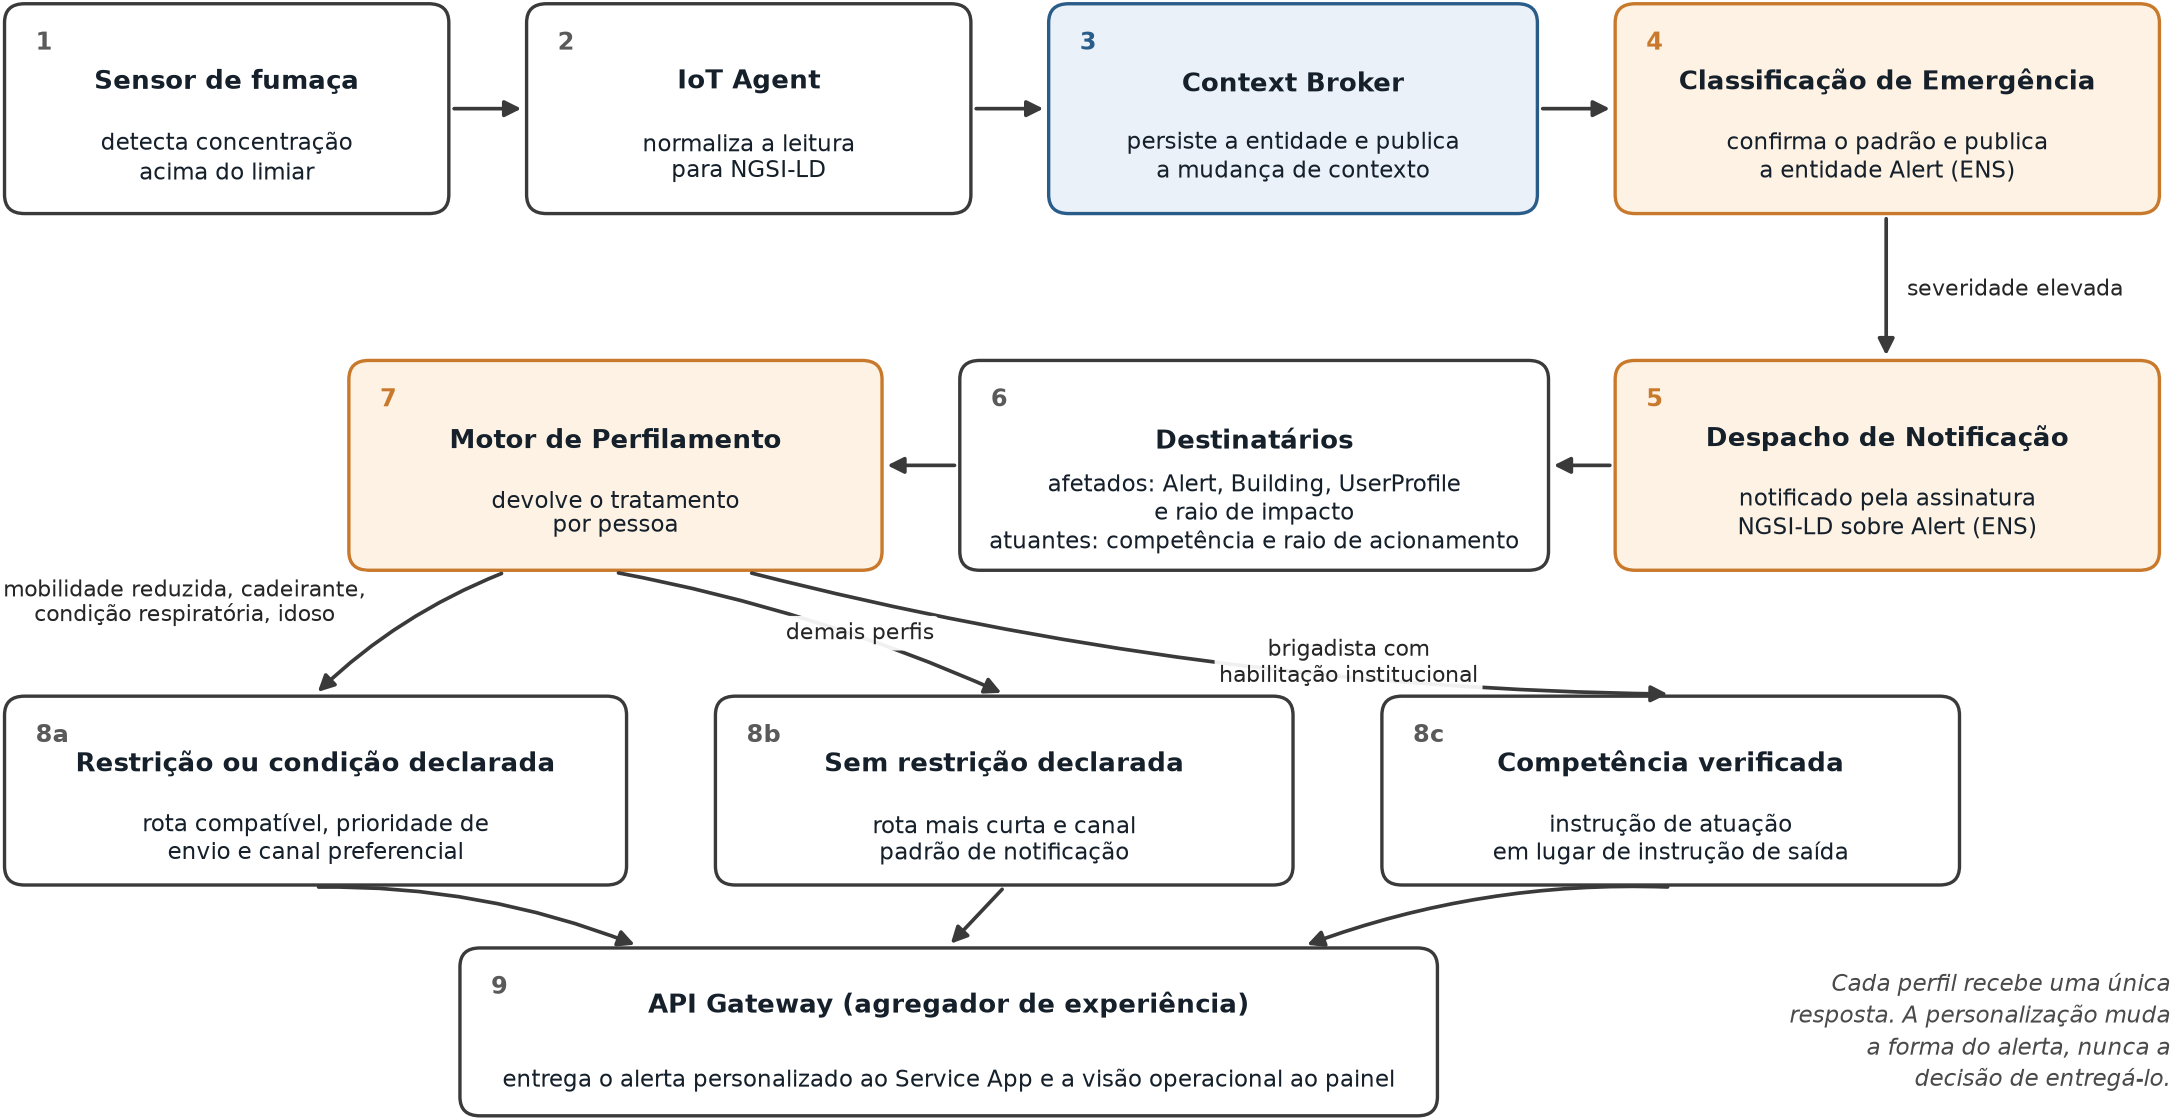
\includegraphics[width=\linewidth]{Imagens/fig_atividades.png}
		\par
		\raggedright
		\footnotesize
		\legend{Fonte: elaborada pelo autor.}
	\end{minipage}
\end{figure}

Um sensor de fumaça em edificação de uso coletivo detecta concentração acima do limiar e reporta a leitura ao agente de dispositivo, que a normaliza para NGSI-LD e a submete ao broker. Validada e persistida a atualização, o \textit{Emergency Classifier} recebe a mudança por assinatura e, confirmado o padrão de incêndio, cria a entidade \texttt{Alert} com severidade elevada e relacionamento \texttt{refersTo} apontando para a edificação.

A criação do alerta satisfaz a assinatura do \textit{Emergency Dispatcher}, que deriva o conjunto afetado combinando a travessia \texttt{Alert}, \texttt{Building}, \texttt{UserProfile} com a consulta geoespacial por raio de impacto, e acrescenta os atuantes pela competência dentro do raio de acionamento. Para cada pessoa do conjunto, o despacho obtém do Motor de Perfilamento o tratamento devido, avaliado contra o escopo de consentimento declarado para a finalidade de resposta a emergência.

As regras são então avaliadas perfil a perfil. Para um cidadão sem restrição declarada, a resposta é o alerta com a rota de saída mais curta pelo canal padrão. Para um cidadão em cadeira de rodas, o cálculo de rota é restrito a segmentos acessíveis e produz itinerário distinto, possivelmente mais longo, porém transitável, e a notificação segue pelo canal sonoro-tátil declarado como preferencial. Para quem declarou condição respiratória ou pertence à faixa etária idosa, o despacho antecipa o envio na fila e a rota prioriza a saída de menor percurso, porque a exposição à fumaça pesa mais nesses casos. \citeonline{deng2022semantic} demonstraram a viabilidade de roteamento sensível às condições do ocupante. O mesmo mecanismo separa também por competência. Um brigadista cuja habilitação tenha sido verificada junto à instituição que a emitiu recebe instrução de atuação em lugar de instrução de saída, esteja ele na edificação ou dentro do raio de acionamento, e o painel de gestão recebe a visão agregada da ocorrência. A diferença importa porque competência que a própria pessoa declara não basta para encarregá-la de resposta a incêndio, e o relacionamento \texttt{providedBy} permite exigir origem institucional nesse caso específico. O mesmo evento urbano produz, portanto, respostas distintas, todas derivadas de atributos que já estão integrados ao grafo da cidade. O \textit{API Gateway} entrega o \textit{payload} à aplicação do cidadão e ao painel de gestão, e a trilha de auditoria registra, por perfil notificado, a regra aplicada e a decisão de autorização que liberou o acesso ao perfil de acessibilidade.

	% \chapter{Estado Atual da Implementação}
TODO
	% \chapter{Plano de Avaliação}
TODO
	% \chapter{Considerações Parciais e Cronograma}
TODO

	% Bibliografia
	\bibliography{Capitulos/Referencias}
	\bibliographystyle{abnt-alf}

	% Pagina em branco
	\newpage

\end{document}
